\documentclass[twoside]{book}

% Packages required by doxygen
\usepackage{fixltx2e}
\usepackage{calc}
\usepackage{doxygen}
\usepackage[export]{adjustbox} % also loads graphicx
\usepackage{graphicx}
\usepackage[utf8]{inputenc}
\usepackage{makeidx}
\usepackage{multicol}
\usepackage{multirow}
\PassOptionsToPackage{warn}{textcomp}
\usepackage{textcomp}
\usepackage[nointegrals]{wasysym}
\usepackage[table]{xcolor}

% NLS support packages
\usepackage{polski}
\usepackage[T1]{fontenc}

% Font selection
\usepackage[T1]{fontenc}
\usepackage[scaled=.90]{helvet}
\usepackage{courier}
\usepackage{amssymb}
\usepackage{sectsty}
\renewcommand{\familydefault}{\sfdefault}
\allsectionsfont{%
  \fontseries{bc}\selectfont%
  \color{darkgray}%
}
\renewcommand{\DoxyLabelFont}{%
  \fontseries{bc}\selectfont%
  \color{darkgray}%
}
\newcommand{\+}{\discretionary{\mbox{\scriptsize$\hookleftarrow$}}{}{}}

% Page & text layout
\usepackage{geometry}
\geometry{%
  a4paper,%
  top=2.5cm,%
  bottom=2.5cm,%
  left=2.5cm,%
  right=2.5cm%
}
\tolerance=750
\hfuzz=15pt
\hbadness=750
\setlength{\emergencystretch}{15pt}
\setlength{\parindent}{0cm}
\setlength{\parskip}{3ex plus 2ex minus 2ex}
\makeatletter
\renewcommand{\paragraph}{%
  \@startsection{paragraph}{4}{0ex}{-1.0ex}{1.0ex}{%
    \normalfont\normalsize\bfseries\SS@parafont%
  }%
}
\renewcommand{\subparagraph}{%
  \@startsection{subparagraph}{5}{0ex}{-1.0ex}{1.0ex}{%
    \normalfont\normalsize\bfseries\SS@subparafont%
  }%
}
\makeatother

% Headers & footers
\usepackage{fancyhdr}
\pagestyle{fancyplain}
\fancyhead[LE]{\fancyplain{}{\bfseries\thepage}}
\fancyhead[CE]{\fancyplain{}{}}
\fancyhead[RE]{\fancyplain{}{\bfseries\leftmark}}
\fancyhead[LO]{\fancyplain{}{\bfseries\rightmark}}
\fancyhead[CO]{\fancyplain{}{}}
\fancyhead[RO]{\fancyplain{}{\bfseries\thepage}}
\fancyfoot[LE]{\fancyplain{}{}}
\fancyfoot[CE]{\fancyplain{}{}}
\fancyfoot[RE]{\fancyplain{}{\bfseries\scriptsize Wygenerowano przez Doxygen }}
\fancyfoot[LO]{\fancyplain{}{\bfseries\scriptsize Wygenerowano przez Doxygen }}
\fancyfoot[CO]{\fancyplain{}{}}
\fancyfoot[RO]{\fancyplain{}{}}
\renewcommand{\footrulewidth}{0.4pt}
\renewcommand{\chaptermark}[1]{%
  \markboth{#1}{}%
}
\renewcommand{\sectionmark}[1]{%
  \markright{\thesection\ #1}%
}

% Indices & bibliography
\usepackage{natbib}
\usepackage[titles]{tocloft}
\setcounter{tocdepth}{3}
\setcounter{secnumdepth}{5}
\makeindex

% Custom commands
\newcommand{\clearemptydoublepage}{%
  \newpage{\pagestyle{empty}\cleardoublepage}%
}

\usepackage{caption}
\captionsetup{labelsep=space,justification=centering,font={bf},singlelinecheck=off,skip=4pt,position=top}

%===== C O N T E N T S =====

\begin{document}

% Titlepage & ToC
\pagenumbering{roman}
\begin{titlepage}
\vspace*{7cm}
\begin{center}%
{\Large Samolot }\\
\vspace*{1cm}
{\large Wygenerowano przez Doxygen 1.8.11}\\
\end{center}
\end{titlepage}
\clearemptydoublepage
\tableofcontents
\clearemptydoublepage
\pagenumbering{arabic}

%--- Begin generated contents ---
\chapter{Indeks hierarchiczny}
\section{Hierarchia klas}
Ta lista dziedziczenia posortowana jest z grubsza, choć nie całkowicie, alfabetycznie\+:\begin{DoxyCompactList}
\item \contentsline{section}{Dane\+Samolotu}{\pageref{class_dane_samolotu}}{}
\item \contentsline{section}{Pasazerowie}{\pageref{class_pasazerowie}}{}
\item \contentsline{section}{Srodek\+\_\+transportu}{\pageref{class_srodek__transportu}}{}
\begin{DoxyCompactList}
\item \contentsline{section}{Samochod}{\pageref{class_samochod}}{}
\item \contentsline{section}{Samolot}{\pageref{class_samolot}}{}
\begin{DoxyCompactList}
\item \contentsline{section}{Samolot\+\_\+wojskowy}{\pageref{class_samolot__wojskowy}}{}
\end{DoxyCompactList}
\end{DoxyCompactList}
\item \contentsline{section}{Zaloga}{\pageref{class_zaloga}}{}
\end{DoxyCompactList}

\chapter{Indeks klas}
\section{Lista klas}
Tutaj znajdują się klasy, struktury, unie i interfejsy wraz z ich krótkimi opisami\+:\begin{DoxyCompactList}
\item\contentsline{section}{{\bf Dane\+Samolotu} \\*Klasa \doxyref{Dane\+Samolotu}{str.}{class_dane_samolotu} }{\pageref{class_dane_samolotu}}{}
\item\contentsline{section}{{\bf Pasazerowie} \\*Klasa \doxyref{Pasazerowie}{str.}{class_pasazerowie} }{\pageref{class_pasazerowie}}{}
\item\contentsline{section}{{\bf Samochod} \\*Klasa \doxyref{Samochod}{str.}{class_samochod}, dziedziczy po klasie \doxyref{Srodek\+\_\+transportu}{str.}{class_srodek__transportu} }{\pageref{class_samochod}}{}
\item\contentsline{section}{{\bf Samolot} \\*Klasa \doxyref{Samolot}{str.}{class_samolot}, dziedziczy po klasie \doxyref{Srodek\+\_\+transportu}{str.}{class_srodek__transportu} }{\pageref{class_samolot}}{}
\item\contentsline{section}{{\bf Samolot\+\_\+wojskowy} \\*Klasa \doxyref{Samolot\+\_\+wojskowy}{str.}{class_samolot__wojskowy}, dziedziczy po klasie \doxyref{Samolot}{str.}{class_samolot} }{\pageref{class_samolot__wojskowy}}{}
\item\contentsline{section}{{\bf Srodek\+\_\+transportu} \\*Klasa abstrakcyjna \doxyref{Srodek\+\_\+transportu}{str.}{class_srodek__transportu} }{\pageref{class_srodek__transportu}}{}
\item\contentsline{section}{{\bf Zaloga} \\*Klasa \doxyref{Zaloga}{str.}{class_zaloga} }{\pageref{class_zaloga}}{}
\end{DoxyCompactList}

\chapter{Indeks plików}
\section{Lista plików}
Tutaj znajduje się lista wszystkich plików z ich krótkimi opisami\+:\begin{DoxyCompactList}
\item\contentsline{section}{{\bf dane\+\_\+samolotu.\+cpp} }{\pageref{dane__samolotu_8cpp}}{}
\item\contentsline{section}{{\bf dane\+\_\+samolotu.\+h} }{\pageref{dane__samolotu_8h}}{}
\item\contentsline{section}{{\bf pasazerowie.\+cpp} }{\pageref{pasazerowie_8cpp}}{}
\item\contentsline{section}{{\bf pasazerowie.\+h} }{\pageref{pasazerowie_8h}}{}
\item\contentsline{section}{{\bf program.\+cpp} }{\pageref{program_8cpp}}{}
\item\contentsline{section}{{\bf samochod.\+cpp} }{\pageref{samochod_8cpp}}{}
\item\contentsline{section}{{\bf samochod.\+h} }{\pageref{samochod_8h}}{}
\item\contentsline{section}{{\bf samolot.\+cpp} }{\pageref{samolot_8cpp}}{}
\item\contentsline{section}{{\bf samolot.\+h} }{\pageref{samolot_8h}}{}
\item\contentsline{section}{{\bf samolot\+\_\+wojskowy.\+cpp} }{\pageref{samolot__wojskowy_8cpp}}{}
\item\contentsline{section}{{\bf samolot\+\_\+wojskowy.\+h} }{\pageref{samolot__wojskowy_8h}}{}
\item\contentsline{section}{{\bf srodek\+\_\+transportu.\+cpp} }{\pageref{srodek__transportu_8cpp}}{}
\item\contentsline{section}{{\bf srodek\+\_\+transportu.\+h} }{\pageref{srodek__transportu_8h}}{}
\item\contentsline{section}{{\bf zaloga.\+cpp} }{\pageref{zaloga_8cpp}}{}
\item\contentsline{section}{{\bf zaloga.\+h} }{\pageref{zaloga_8h}}{}
\end{DoxyCompactList}

\chapter{Dokumentacja klas}
\section{Dokumentacja klasy Dane\+Samolotu}
\label{class_dane_samolotu}\index{Dane\+Samolotu@{Dane\+Samolotu}}


klasa \doxyref{Dane\+Samolotu}{str.}{class_dane_samolotu}  




{\ttfamily \#include $<$dane\+\_\+samolotu.\+h$>$}

\subsection*{Metody publiczne}
\begin{DoxyCompactItemize}
\item 
{\bf Dane\+Samolotu} ()
\begin{DoxyCompactList}\small\item\em konstruktor domyslny \end{DoxyCompactList}\item 
{\bf $\sim$\+Dane\+Samolotu} ()
\begin{DoxyCompactList}\small\item\em destruktor \end{DoxyCompactList}\item 
void {\bf zwrocdane} ()
\begin{DoxyCompactList}\small\item\em metoda zwracajace start i cel lotu \end{DoxyCompactList}\item 
void {\bf zmiendane} (string nowystart, string nowycel)
\begin{DoxyCompactList}\small\item\em metoda umozliwiajaca zmiane danych lotu \end{DoxyCompactList}\item 
{\bf Dane\+Samolotu} \& {\bf operator=} (const {\bf Dane\+Samolotu} \&dane)
\begin{DoxyCompactList}\small\item\em przeciazony operator = \end{DoxyCompactList}\end{DoxyCompactItemize}
\subsection*{Przyjaciele}
\begin{DoxyCompactItemize}
\item 
ostream \& {\bf operator$<$$<$} (ostream \&out, {\bf Dane\+Samolotu} \&dane)
\begin{DoxyCompactList}\small\item\em Operator strumieniowy $<$$<$. \end{DoxyCompactList}\item 
istream \& {\bf operator$>$$>$} (istream \&s, {\bf Dane\+Samolotu} \&dane)
\begin{DoxyCompactList}\small\item\em Operator strumieniowy $>$$>$ \end{DoxyCompactList}\end{DoxyCompactItemize}


\subsection{Opis szczegółowy}
klasa \doxyref{Dane\+Samolotu}{str.}{class_dane_samolotu} 

\subsection{Dokumentacja konstruktora i destruktora}
\index{Dane\+Samolotu@{Dane\+Samolotu}!Dane\+Samolotu@{Dane\+Samolotu}}
\index{Dane\+Samolotu@{Dane\+Samolotu}!Dane\+Samolotu@{Dane\+Samolotu}}
\subsubsection[{Dane\+Samolotu()}]{\setlength{\rightskip}{0pt plus 5cm}Dane\+Samolotu\+::\+Dane\+Samolotu (
\begin{DoxyParamCaption}
{}
\end{DoxyParamCaption}
)}\label{class_dane_samolotu_a884d0e9aa3ee5c89f67fea4d765f485c}


konstruktor domyslny 

\index{Dane\+Samolotu@{Dane\+Samolotu}!````~Dane\+Samolotu@{$\sim$\+Dane\+Samolotu}}
\index{````~Dane\+Samolotu@{$\sim$\+Dane\+Samolotu}!Dane\+Samolotu@{Dane\+Samolotu}}
\subsubsection[{$\sim$\+Dane\+Samolotu()}]{\setlength{\rightskip}{0pt plus 5cm}Dane\+Samolotu\+::$\sim$\+Dane\+Samolotu (
\begin{DoxyParamCaption}
{}
\end{DoxyParamCaption}
)}\label{class_dane_samolotu_ad11362e0176afdcad05918f7525af4ec}


destruktor 



\subsection{Dokumentacja funkcji składowych}
\index{Dane\+Samolotu@{Dane\+Samolotu}!operator=@{operator=}}
\index{operator=@{operator=}!Dane\+Samolotu@{Dane\+Samolotu}}
\subsubsection[{operator=(const Dane\+Samolotu \&dane)}]{\setlength{\rightskip}{0pt plus 5cm}{\bf Dane\+Samolotu} \& Dane\+Samolotu\+::operator= (
\begin{DoxyParamCaption}
\item[{const {\bf Dane\+Samolotu} \&}]{dane}
\end{DoxyParamCaption}
)}\label{class_dane_samolotu_af79dbd14f7579abf44221ebdc5d629fd}


przeciazony operator = 

\index{Dane\+Samolotu@{Dane\+Samolotu}!zmiendane@{zmiendane}}
\index{zmiendane@{zmiendane}!Dane\+Samolotu@{Dane\+Samolotu}}
\subsubsection[{zmiendane(string nowystart, string nowycel)}]{\setlength{\rightskip}{0pt plus 5cm}void Dane\+Samolotu\+::zmiendane (
\begin{DoxyParamCaption}
\item[{string}]{nowystart, }
\item[{string}]{nowycel}
\end{DoxyParamCaption}
)}\label{class_dane_samolotu_a83409c2502884bb0f87dd70eb2ea60d9}


metoda umozliwiajaca zmiane danych lotu 

umozliwia ustawienie nowego miejsca startu i celu lotu 
\begin{DoxyParams}{Parametry}
{\em nowystart} & to miejsce nowego startu lotu \\
\hline
{\em nowycel} & to miejsce nowego celu lotu \\
\hline
\end{DoxyParams}
\begin{DoxyReturn}{Zwraca}
nic nie zwraca 
\end{DoxyReturn}
\index{Dane\+Samolotu@{Dane\+Samolotu}!zwrocdane@{zwrocdane}}
\index{zwrocdane@{zwrocdane}!Dane\+Samolotu@{Dane\+Samolotu}}
\subsubsection[{zwrocdane()}]{\setlength{\rightskip}{0pt plus 5cm}void Dane\+Samolotu\+::zwrocdane (
\begin{DoxyParamCaption}
{}
\end{DoxyParamCaption}
)}\label{class_dane_samolotu_a2dfa2684ef2b7b6228e730924f90d2dd}


metoda zwracajace start i cel lotu 



\subsection{Dokumentacja przyjaciół i funkcji związanych}
\index{Dane\+Samolotu@{Dane\+Samolotu}!operator$<$$<$@{operator$<$$<$}}
\index{operator$<$$<$@{operator$<$$<$}!Dane\+Samolotu@{Dane\+Samolotu}}
\subsubsection[{operator$<$$<$}]{\setlength{\rightskip}{0pt plus 5cm}ostream\& operator$<$$<$ (
\begin{DoxyParamCaption}
\item[{ostream \&}]{out, }
\item[{{\bf Dane\+Samolotu} \&}]{dane}
\end{DoxyParamCaption}
)\hspace{0.3cm}{\ttfamily [friend]}}\label{class_dane_samolotu_aaaf6a3db89522d407cf92091a98c2e80}


Operator strumieniowy $<$$<$. 

\index{Dane\+Samolotu@{Dane\+Samolotu}!operator$>$$>$@{operator$>$$>$}}
\index{operator$>$$>$@{operator$>$$>$}!Dane\+Samolotu@{Dane\+Samolotu}}
\subsubsection[{operator$>$$>$}]{\setlength{\rightskip}{0pt plus 5cm}istream\& operator$>$$>$ (
\begin{DoxyParamCaption}
\item[{istream \&}]{s, }
\item[{{\bf Dane\+Samolotu} \&}]{dane}
\end{DoxyParamCaption}
)\hspace{0.3cm}{\ttfamily [friend]}}\label{class_dane_samolotu_ae1a66a9e4246344008e3874910e3045d}


Operator strumieniowy $>$$>$ 



Dokumentacja dla tej klasy została wygenerowana z plików\+:\begin{DoxyCompactItemize}
\item 
{\bf dane\+\_\+samolotu.\+h}\item 
{\bf dane\+\_\+samolotu.\+cpp}\end{DoxyCompactItemize}

\section{Dokumentacja klasy Pasazerowie}
\label{class_pasazerowie}\index{Pasazerowie@{Pasazerowie}}


klasa \doxyref{Pasazerowie}{str.}{class_pasazerowie}  




{\ttfamily \#include $<$pasazerowie.\+h$>$}

\subsection*{Metody publiczne}
\begin{DoxyCompactItemize}
\item 
{\bf Pasazerowie} ()
\begin{DoxyCompactList}\small\item\em konstruktor domyslny \end{DoxyCompactList}\item 
{\bf $\sim$\+Pasazerowie} ()
\begin{DoxyCompactList}\small\item\em destruktor \end{DoxyCompactList}\item 
string {\bf zwrocimie} ()
\begin{DoxyCompactList}\small\item\em metoda zwracajaca imie \end{DoxyCompactList}\item 
string {\bf zwrocnazwisko} ()
\begin{DoxyCompactList}\small\item\em metoda zwracajaca nazwisko \end{DoxyCompactList}\item 
void {\bf calanazwa} ()
\begin{DoxyCompactList}\small\item\em metoda wypisujaca ��cznie imie i nazwisko \end{DoxyCompactList}\item 
void {\bf zmienimie} (string noweimie)
\begin{DoxyCompactList}\small\item\em metoda pozwalajaca na zmiane imienia \end{DoxyCompactList}\item 
void {\bf zmiennazwisko} (string nowenazwisko)
\begin{DoxyCompactList}\small\item\em metoda pozwalajaca na zmiane nazwiska \end{DoxyCompactList}\item 
void {\bf zwrocnadbagaz} ()
\begin{DoxyCompactList}\small\item\em metoda zwracajaca informacje czy pasazer posiada nadbagaz \end{DoxyCompactList}\item 
void {\bf operator!} ()
\begin{DoxyCompactList}\small\item\em przeciazony operator ! \end{DoxyCompactList}\end{DoxyCompactItemize}
\subsection*{Przyjaciele}
\begin{DoxyCompactItemize}
\item 
ostream \& {\bf operator$<$$<$} (ostream \&out, {\bf Pasazerowie} \&pasazerowie)
\begin{DoxyCompactList}\small\item\em Operator strumieniowy $<$$<$. \end{DoxyCompactList}\item 
istream \& {\bf operator$>$$>$} (istream \&s, {\bf Pasazerowie} \&pasazerowie)
\begin{DoxyCompactList}\small\item\em Operator strumieniowy $>$$>$ \end{DoxyCompactList}\end{DoxyCompactItemize}


\subsection{Opis szczegółowy}
klasa \doxyref{Pasazerowie}{str.}{class_pasazerowie} 

\subsection{Dokumentacja konstruktora i destruktora}
\index{Pasazerowie@{Pasazerowie}!Pasazerowie@{Pasazerowie}}
\index{Pasazerowie@{Pasazerowie}!Pasazerowie@{Pasazerowie}}
\subsubsection[{Pasazerowie()}]{\setlength{\rightskip}{0pt plus 5cm}Pasazerowie\+::\+Pasazerowie (
\begin{DoxyParamCaption}
{}
\end{DoxyParamCaption}
)}\label{class_pasazerowie_a1389ee395e17bb6bb0794da800a31706}


konstruktor domyslny 

\index{Pasazerowie@{Pasazerowie}!````~Pasazerowie@{$\sim$\+Pasazerowie}}
\index{````~Pasazerowie@{$\sim$\+Pasazerowie}!Pasazerowie@{Pasazerowie}}
\subsubsection[{$\sim$\+Pasazerowie()}]{\setlength{\rightskip}{0pt plus 5cm}Pasazerowie\+::$\sim$\+Pasazerowie (
\begin{DoxyParamCaption}
{}
\end{DoxyParamCaption}
)}\label{class_pasazerowie_ad655ce26cdb3b1ff72363ca0dbbb79d3}


destruktor 



\subsection{Dokumentacja funkcji składowych}
\index{Pasazerowie@{Pasazerowie}!calanazwa@{calanazwa}}
\index{calanazwa@{calanazwa}!Pasazerowie@{Pasazerowie}}
\subsubsection[{calanazwa()}]{\setlength{\rightskip}{0pt plus 5cm}void Pasazerowie\+::calanazwa (
\begin{DoxyParamCaption}
{}
\end{DoxyParamCaption}
)}\label{class_pasazerowie_ab9edddcbd33a81cf1574ccdcb4e61eb5}


metoda wypisujaca ��cznie imie i nazwisko 

\index{Pasazerowie@{Pasazerowie}!operator"!@{operator"!}}
\index{operator"!@{operator"!}!Pasazerowie@{Pasazerowie}}
\subsubsection[{operator"!()}]{\setlength{\rightskip}{0pt plus 5cm}void Pasazerowie\+::operator! (
\begin{DoxyParamCaption}
{}
\end{DoxyParamCaption}
)}\label{class_pasazerowie_a82b3004cb658596a226c94e21336afff}


przeciazony operator ! 

\index{Pasazerowie@{Pasazerowie}!zmienimie@{zmienimie}}
\index{zmienimie@{zmienimie}!Pasazerowie@{Pasazerowie}}
\subsubsection[{zmienimie(string noweimie)}]{\setlength{\rightskip}{0pt plus 5cm}void Pasazerowie\+::zmienimie (
\begin{DoxyParamCaption}
\item[{string}]{noweimie}
\end{DoxyParamCaption}
)}\label{class_pasazerowie_a18547974c389d9c4e05a514195c293de}


metoda pozwalajaca na zmiane imienia 


\begin{DoxyParams}{Parametry}
{\em noweimie} & to nowe imie pasazera \\
\hline
\end{DoxyParams}
\begin{DoxyReturn}{Zwraca}
nic nie zwraca 
\end{DoxyReturn}
\index{Pasazerowie@{Pasazerowie}!zmiennazwisko@{zmiennazwisko}}
\index{zmiennazwisko@{zmiennazwisko}!Pasazerowie@{Pasazerowie}}
\subsubsection[{zmiennazwisko(string nowenazwisko)}]{\setlength{\rightskip}{0pt plus 5cm}void Pasazerowie\+::zmiennazwisko (
\begin{DoxyParamCaption}
\item[{string}]{nowenazwisko}
\end{DoxyParamCaption}
)}\label{class_pasazerowie_a13533bd4bc2fb36c11513cb5f71b686e}


metoda pozwalajaca na zmiane nazwiska 


\begin{DoxyParams}{Parametry}
{\em nowenazwisko} & to nowe nazwisko pasazera \\
\hline
\end{DoxyParams}
\begin{DoxyReturn}{Zwraca}
nic nie zwraca 
\end{DoxyReturn}
\index{Pasazerowie@{Pasazerowie}!zwrocimie@{zwrocimie}}
\index{zwrocimie@{zwrocimie}!Pasazerowie@{Pasazerowie}}
\subsubsection[{zwrocimie()}]{\setlength{\rightskip}{0pt plus 5cm}string Pasazerowie\+::zwrocimie (
\begin{DoxyParamCaption}
{}
\end{DoxyParamCaption}
)}\label{class_pasazerowie_a15bbfaafc3a7b7f473dd7cbbb2c41bef}


metoda zwracajaca imie 

\begin{DoxyReturn}{Zwraca}
zwraca imie pasazera 
\end{DoxyReturn}
\index{Pasazerowie@{Pasazerowie}!zwrocnadbagaz@{zwrocnadbagaz}}
\index{zwrocnadbagaz@{zwrocnadbagaz}!Pasazerowie@{Pasazerowie}}
\subsubsection[{zwrocnadbagaz()}]{\setlength{\rightskip}{0pt plus 5cm}void Pasazerowie\+::zwrocnadbagaz (
\begin{DoxyParamCaption}
{}
\end{DoxyParamCaption}
)}\label{class_pasazerowie_abf88517c867095015640c7faffdee03a}


metoda zwracajaca informacje czy pasazer posiada nadbagaz 

\index{Pasazerowie@{Pasazerowie}!zwrocnazwisko@{zwrocnazwisko}}
\index{zwrocnazwisko@{zwrocnazwisko}!Pasazerowie@{Pasazerowie}}
\subsubsection[{zwrocnazwisko()}]{\setlength{\rightskip}{0pt plus 5cm}string Pasazerowie\+::zwrocnazwisko (
\begin{DoxyParamCaption}
{}
\end{DoxyParamCaption}
)}\label{class_pasazerowie_a3367047420d01fe7ea90563054bb4227}


metoda zwracajaca nazwisko 

\begin{DoxyReturn}{Zwraca}
zwraca nazwisko pasazera 
\end{DoxyReturn}


\subsection{Dokumentacja przyjaciół i funkcji związanych}
\index{Pasazerowie@{Pasazerowie}!operator$<$$<$@{operator$<$$<$}}
\index{operator$<$$<$@{operator$<$$<$}!Pasazerowie@{Pasazerowie}}
\subsubsection[{operator$<$$<$}]{\setlength{\rightskip}{0pt plus 5cm}ostream\& operator$<$$<$ (
\begin{DoxyParamCaption}
\item[{ostream \&}]{out, }
\item[{{\bf Pasazerowie} \&}]{pasazerowie}
\end{DoxyParamCaption}
)\hspace{0.3cm}{\ttfamily [friend]}}\label{class_pasazerowie_a2450aa552025411d4775ec11a1d091d2}


Operator strumieniowy $<$$<$. 

\index{Pasazerowie@{Pasazerowie}!operator$>$$>$@{operator$>$$>$}}
\index{operator$>$$>$@{operator$>$$>$}!Pasazerowie@{Pasazerowie}}
\subsubsection[{operator$>$$>$}]{\setlength{\rightskip}{0pt plus 5cm}istream\& operator$>$$>$ (
\begin{DoxyParamCaption}
\item[{istream \&}]{s, }
\item[{{\bf Pasazerowie} \&}]{pasazerowie}
\end{DoxyParamCaption}
)\hspace{0.3cm}{\ttfamily [friend]}}\label{class_pasazerowie_a42b7ff0865bca4ed3d43a45b68c7bcdd}


Operator strumieniowy $>$$>$ 



Dokumentacja dla tej klasy została wygenerowana z plików\+:\begin{DoxyCompactItemize}
\item 
{\bf pasazerowie.\+h}\item 
{\bf pasazerowie.\+cpp}\end{DoxyCompactItemize}

\section{Dokumentacja klasy Samochod}
\label{class_samochod}\index{Samochod@{Samochod}}


Klasa \doxyref{Samochod}{str.}{class_samochod}, dziedziczy po klasie \doxyref{Srodek\+\_\+transportu}{str.}{class_srodek__transportu}.  




{\ttfamily \#include $<$samochod.\+h$>$}

Diagram dziedziczenia dla Samochod\begin{figure}[H]
\begin{center}
\leavevmode
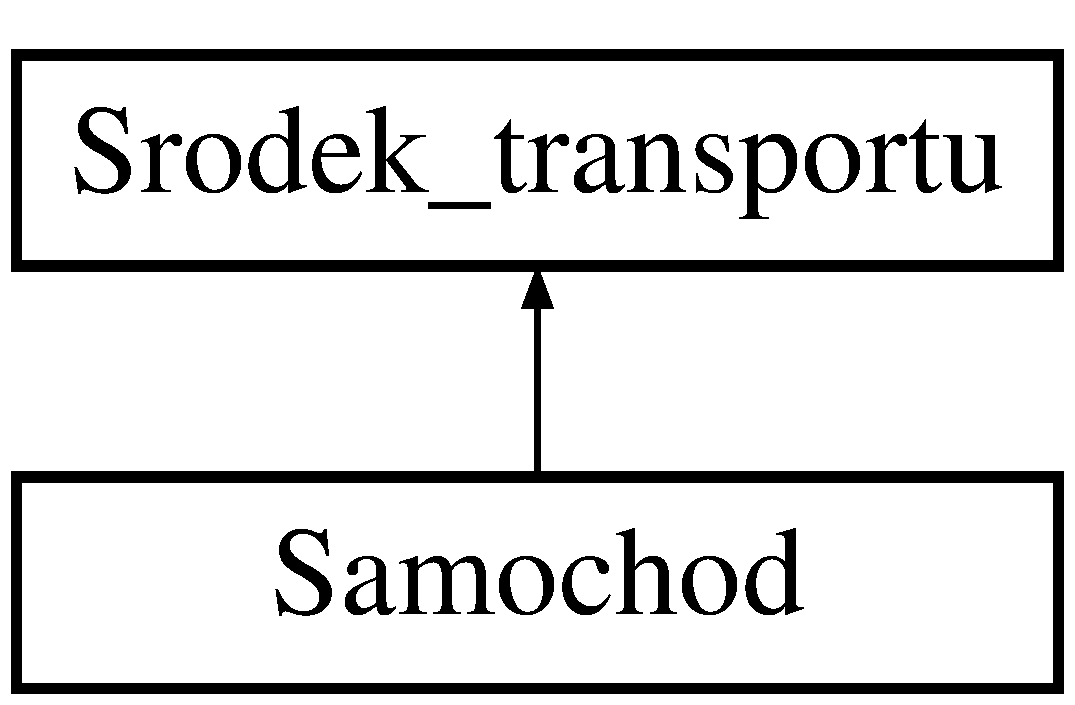
\includegraphics[height=2.000000cm]{class_samochod}
\end{center}
\end{figure}
\subsection*{Metody publiczne}
\begin{DoxyCompactItemize}
\item 
{\bf Samochod} ()
\begin{DoxyCompactList}\small\item\em konstruktor domyslny \end{DoxyCompactList}\item 
{\bf $\sim$\+Samochod} ()
\begin{DoxyCompactList}\small\item\em destruktor \end{DoxyCompactList}\item 
void {\bf zapisz\+\_\+samochod} (string nazwa)
\begin{DoxyCompactList}\small\item\em funkcja zapisu do pliku zmiennych z klasy samochod \end{DoxyCompactList}\item 
void {\bf wczytaj\+\_\+samochod} (string nazwa)
\begin{DoxyCompactList}\small\item\em funkcja odczytu z pliku zmiennych z klasy samochod \end{DoxyCompactList}\item 
virtual void {\bf wypisz\+\_\+stan} ()
\begin{DoxyCompactList}\small\item\em funkcja wypisujaca stan samochodu \end{DoxyCompactList}\item 
virtual void {\bf ustaw\+\_\+domyslne} ()
\begin{DoxyCompactList}\small\item\em funkcja ustawiajaca parametry domyslne samochodu \end{DoxyCompactList}\end{DoxyCompactItemize}
\subsection*{Atrybuty chronione}
\begin{DoxyCompactItemize}
\item 
int {\bf przebieg}
\begin{DoxyCompactList}\small\item\em zmienna przechowuj�ca przebieg \end{DoxyCompactList}\end{DoxyCompactItemize}
\subsection*{Przyjaciele}
\begin{DoxyCompactItemize}
\item 
ostream \& {\bf operator$<$$<$} (ostream \&out, {\bf Samochod} \&samochod)
\begin{DoxyCompactList}\small\item\em Operator strumieniowy $<$$<$. \end{DoxyCompactList}\item 
istream \& {\bf operator$>$$>$} (istream \&s, {\bf Samochod} \&samochod)
\begin{DoxyCompactList}\small\item\em Operator strumieniowy $>$$>$ \end{DoxyCompactList}\end{DoxyCompactItemize}


\subsection{Opis szczegółowy}
Klasa \doxyref{Samochod}{str.}{class_samochod}, dziedziczy po klasie \doxyref{Srodek\+\_\+transportu}{str.}{class_srodek__transportu}. 

\subsection{Dokumentacja konstruktora i destruktora}
\index{Samochod@{Samochod}!Samochod@{Samochod}}
\index{Samochod@{Samochod}!Samochod@{Samochod}}
\subsubsection[{Samochod()}]{\setlength{\rightskip}{0pt plus 5cm}Samochod\+::\+Samochod (
\begin{DoxyParamCaption}
{}
\end{DoxyParamCaption}
)}\label{class_samochod_a56ae27a3e568333f010604249d463c96}


konstruktor domyslny 

\index{Samochod@{Samochod}!````~Samochod@{$\sim$\+Samochod}}
\index{````~Samochod@{$\sim$\+Samochod}!Samochod@{Samochod}}
\subsubsection[{$\sim$\+Samochod()}]{\setlength{\rightskip}{0pt plus 5cm}Samochod\+::$\sim$\+Samochod (
\begin{DoxyParamCaption}
{}
\end{DoxyParamCaption}
)}\label{class_samochod_a5995c359256c60addb4b362c2797b37c}


destruktor 



\subsection{Dokumentacja funkcji składowych}
\index{Samochod@{Samochod}!ustaw\+\_\+domyslne@{ustaw\+\_\+domyslne}}
\index{ustaw\+\_\+domyslne@{ustaw\+\_\+domyslne}!Samochod@{Samochod}}
\subsubsection[{ustaw\+\_\+domyslne()}]{\setlength{\rightskip}{0pt plus 5cm}void Samochod\+::ustaw\+\_\+domyslne (
\begin{DoxyParamCaption}
{}
\end{DoxyParamCaption}
)\hspace{0.3cm}{\ttfamily [virtual]}}\label{class_samochod_affb67e0cc339a6fe027a82703dc4c0e9}


funkcja ustawiajaca parametry domyslne samochodu 



Implementuje {\bf Srodek\+\_\+transportu} \doxyref{}{str.}{class_srodek__transportu_a001cdf92b562557afa60257d174d524b}.

\index{Samochod@{Samochod}!wczytaj\+\_\+samochod@{wczytaj\+\_\+samochod}}
\index{wczytaj\+\_\+samochod@{wczytaj\+\_\+samochod}!Samochod@{Samochod}}
\subsubsection[{wczytaj\+\_\+samochod(string nazwa)}]{\setlength{\rightskip}{0pt plus 5cm}void Samochod\+::wczytaj\+\_\+samochod (
\begin{DoxyParamCaption}
\item[{string}]{nazwa}
\end{DoxyParamCaption}
)}\label{class_samochod_ae7dad1c2a66fb7a7605f3326f1008926}


funkcja odczytu z pliku zmiennych z klasy samochod 


\begin{DoxyParams}{Parametry}
{\em nazwa} & to nazwa pliku txt \\
\hline
\end{DoxyParams}
\index{Samochod@{Samochod}!wypisz\+\_\+stan@{wypisz\+\_\+stan}}
\index{wypisz\+\_\+stan@{wypisz\+\_\+stan}!Samochod@{Samochod}}
\subsubsection[{wypisz\+\_\+stan()}]{\setlength{\rightskip}{0pt plus 5cm}void Samochod\+::wypisz\+\_\+stan (
\begin{DoxyParamCaption}
{}
\end{DoxyParamCaption}
)\hspace{0.3cm}{\ttfamily [virtual]}}\label{class_samochod_a45373f78f0764700a4eed0b34c300915}


funkcja wypisujaca stan samochodu 



Implementuje {\bf Srodek\+\_\+transportu} \doxyref{}{str.}{class_srodek__transportu_aed5cfb50e521972271e878d947d7cc5c}.

\index{Samochod@{Samochod}!zapisz\+\_\+samochod@{zapisz\+\_\+samochod}}
\index{zapisz\+\_\+samochod@{zapisz\+\_\+samochod}!Samochod@{Samochod}}
\subsubsection[{zapisz\+\_\+samochod(string nazwa)}]{\setlength{\rightskip}{0pt plus 5cm}void Samochod\+::zapisz\+\_\+samochod (
\begin{DoxyParamCaption}
\item[{string}]{nazwa}
\end{DoxyParamCaption}
)}\label{class_samochod_a346bdce9104f655e7b3d9b58dbd56614}


funkcja zapisu do pliku zmiennych z klasy samochod 


\begin{DoxyParams}{Parametry}
{\em nazwa} & to nazwa pliku txt \\
\hline
\end{DoxyParams}


\subsection{Dokumentacja przyjaciół i funkcji związanych}
\index{Samochod@{Samochod}!operator$<$$<$@{operator$<$$<$}}
\index{operator$<$$<$@{operator$<$$<$}!Samochod@{Samochod}}
\subsubsection[{operator$<$$<$}]{\setlength{\rightskip}{0pt plus 5cm}ostream\& operator$<$$<$ (
\begin{DoxyParamCaption}
\item[{ostream \&}]{out, }
\item[{{\bf Samochod} \&}]{samochod}
\end{DoxyParamCaption}
)\hspace{0.3cm}{\ttfamily [friend]}}\label{class_samochod_a48c7afb882b656c44f52e8a92c26a34b}


Operator strumieniowy $<$$<$. 

\index{Samochod@{Samochod}!operator$>$$>$@{operator$>$$>$}}
\index{operator$>$$>$@{operator$>$$>$}!Samochod@{Samochod}}
\subsubsection[{operator$>$$>$}]{\setlength{\rightskip}{0pt plus 5cm}istream\& operator$>$$>$ (
\begin{DoxyParamCaption}
\item[{istream \&}]{s, }
\item[{{\bf Samochod} \&}]{samochod}
\end{DoxyParamCaption}
)\hspace{0.3cm}{\ttfamily [friend]}}\label{class_samochod_a2ee8222931a9b95803d5a280ebe8ee96}


Operator strumieniowy $>$$>$ 



\subsection{Dokumentacja atrybutów składowych}
\index{Samochod@{Samochod}!przebieg@{przebieg}}
\index{przebieg@{przebieg}!Samochod@{Samochod}}
\subsubsection[{przebieg}]{\setlength{\rightskip}{0pt plus 5cm}int Samochod\+::przebieg\hspace{0.3cm}{\ttfamily [protected]}}\label{class_samochod_ac49f2eb837bb3defec37f573bb39e059}


zmienna przechowuj�ca przebieg 



Dokumentacja dla tej klasy została wygenerowana z plików\+:\begin{DoxyCompactItemize}
\item 
{\bf samochod.\+h}\item 
{\bf samochod.\+cpp}\end{DoxyCompactItemize}

\section{Dokumentacja klasy Samolot}
\label{class_samolot}\index{Samolot@{Samolot}}


Klasa \doxyref{Samolot}{str.}{class_samolot}, dziedziczy po klasie \doxyref{Srodek\+\_\+transportu}{str.}{class_srodek__transportu}.  




{\ttfamily \#include $<$samolot.\+h$>$}

Diagram dziedziczenia dla Samolot\begin{figure}[H]
\begin{center}
\leavevmode
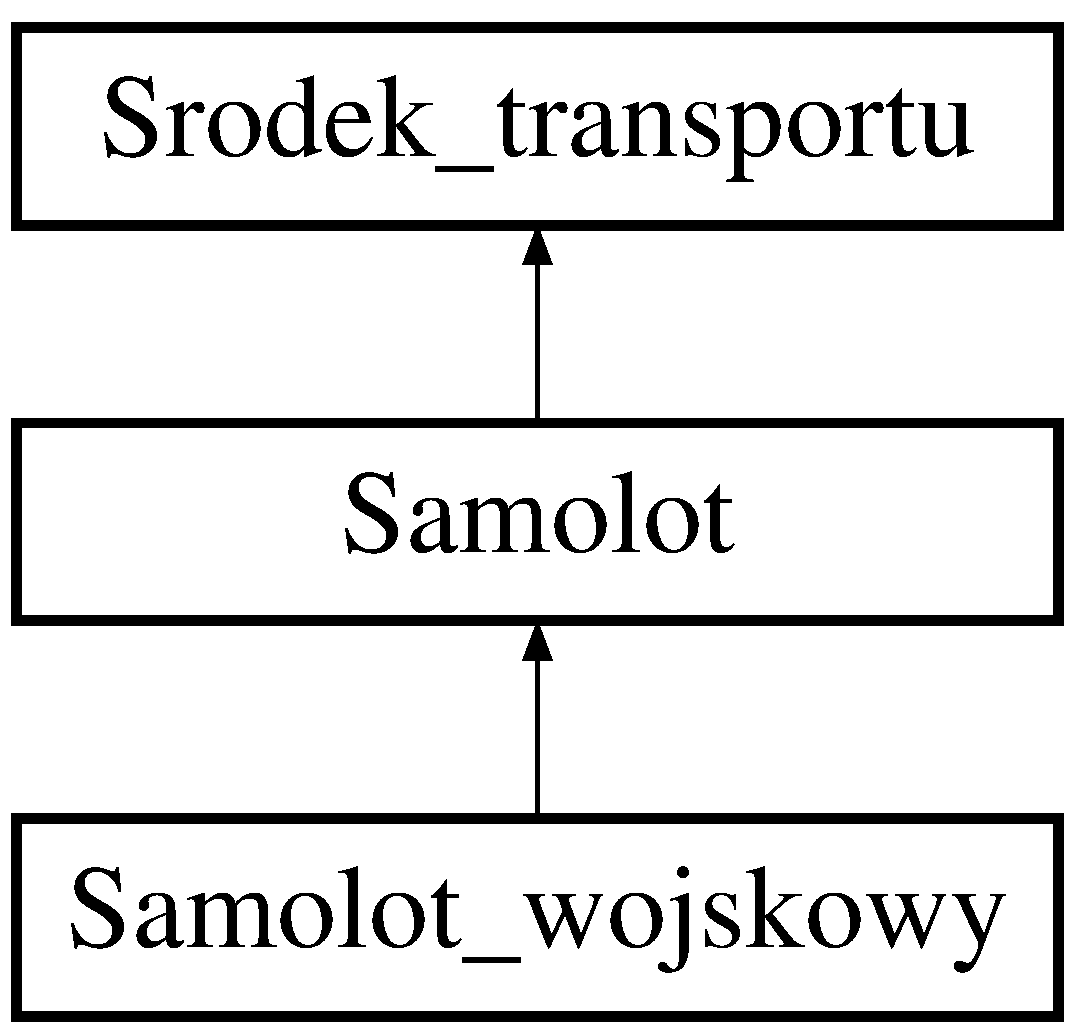
\includegraphics[height=3.000000cm]{class_samolot}
\end{center}
\end{figure}
\subsection*{Metody publiczne}
\begin{DoxyCompactItemize}
\item 
{\bf Samolot} ()
\begin{DoxyCompactList}\small\item\em konstruktor domyslny \end{DoxyCompactList}\item 
{\bf Samolot} (int miejsca, int ilosc\+\_\+osob)
\begin{DoxyCompactList}\small\item\em konstruktor z parametrami \end{DoxyCompactList}\item 
{\bf Samolot} ({\bf Samolot} \&samolot)
\begin{DoxyCompactList}\small\item\em konstruktor kopiujacy \end{DoxyCompactList}\item 
{\bf $\sim$\+Samolot} ()
\begin{DoxyCompactList}\small\item\em destruktor \end{DoxyCompactList}\item 
void {\bf zwroc\+\_\+iloscmiejsc} ()
\begin{DoxyCompactList}\small\item\em metoda zwracajaca ilosc miejsc w samolocie \end{DoxyCompactList}\item 
void {\bf zmienilosc} (int nowailosc)
\begin{DoxyCompactList}\small\item\em metoda z parametrem zmieniajaca ilosc miejsc w smolocie \end{DoxyCompactList}\item 
void {\bf zapisz\+\_\+samolot} (string nazwa)
\begin{DoxyCompactList}\small\item\em funkcja zapisu do pliku zmiennych z klasy samolot \end{DoxyCompactList}\item 
void {\bf wczytaj\+\_\+samolot} (string nazwa)
\begin{DoxyCompactList}\small\item\em funkcja odczytu z pliku zmiennych z klasy samolot \end{DoxyCompactList}\item 
virtual void {\bf wypisz\+\_\+stan} ()
\begin{DoxyCompactList}\small\item\em funkcja wypisujaca stan samolotu \end{DoxyCompactList}\item 
virtual void {\bf ustaw\+\_\+domyslne} ()
\begin{DoxyCompactList}\small\item\em funkcja wirtualna ustawiajaca parametry domyslne samolotu \end{DoxyCompactList}\item 
bool {\bf operator$>$} (const {\bf Samolot} \&samolot)
\begin{DoxyCompactList}\small\item\em przeciazony operator $>$ \end{DoxyCompactList}\item 
bool {\bf operator$<$} (const {\bf Samolot} \&samolot)
\begin{DoxyCompactList}\small\item\em przeciazony operator $<$ \end{DoxyCompactList}\item 
int {\bf operator+} (const {\bf Samolot} \&samolot)
\begin{DoxyCompactList}\small\item\em przeciazony operator + \end{DoxyCompactList}\item 
{\bf operator int} () const 
\begin{DoxyCompactList}\small\item\em przeciazony operator () \end{DoxyCompactList}\item 
{\bf Samolot} \& {\bf operator++} (int)
\begin{DoxyCompactList}\small\item\em przeciazony operator ++ \end{DoxyCompactList}\item 
{\bf Samolot} \& {\bf operator-\/-\/} (int)
\begin{DoxyCompactList}\small\item\em przeciazony operator -- \end{DoxyCompactList}\item 
{\bf Pasazerowie} \& {\bf operator[$\,$]} (int pozycja)
\begin{DoxyCompactList}\small\item\em przeciazony operator [] \end{DoxyCompactList}\item 
{\bf Samolot} \& {\bf operator=} (const {\bf Samolot} \&samolot)
\begin{DoxyCompactList}\small\item\em przeciazony operator = \end{DoxyCompactList}\end{DoxyCompactItemize}
\subsection*{Statyczne metody publiczne}
\begin{DoxyCompactItemize}
\item 
static void {\bf statycznametoda} ()
\begin{DoxyCompactList}\small\item\em metoda statyczna wyswietlajaca ilosc stworzonych obiektow samolot \end{DoxyCompactList}\end{DoxyCompactItemize}
\subsection*{Atrybuty chronione}
\begin{DoxyCompactItemize}
\item 
{\bf Zaloga} {\bf zaloga}
\begin{DoxyCompactList}\small\item\em Podklasa klasy samolot. \end{DoxyCompactList}\item 
{\bf Dane\+Samolotu} {\bf dane\+Samolotu}
\begin{DoxyCompactList}\small\item\em Podklasa klasy samolot. \end{DoxyCompactList}\item 
float {\bf max\+\_\+wysokosc}
\begin{DoxyCompactList}\small\item\em zmienna przechowujaca maksymalna wysokosc lotu \end{DoxyCompactList}\end{DoxyCompactItemize}
\subsection*{Statyczne atrybuty chronione}
\begin{DoxyCompactItemize}
\item 
static int {\bf liczba\+\_\+obiektow} = 0
\begin{DoxyCompactList}\small\item\em zmienna przechowujaca liczbe stworzonych obiektow samolot \end{DoxyCompactList}\end{DoxyCompactItemize}
\subsection*{Przyjaciele}
\begin{DoxyCompactItemize}
\item 
ostream \& {\bf operator$<$$<$} (ostream \&out, {\bf Samolot} \&samolot)
\begin{DoxyCompactList}\small\item\em Operator strumieniowy $<$$<$. \end{DoxyCompactList}\item 
istream \& {\bf operator$>$$>$} (istream \&s, {\bf Samolot} \&samolot)
\begin{DoxyCompactList}\small\item\em Operator strumieniowy $>$$>$ \end{DoxyCompactList}\end{DoxyCompactItemize}


\subsection{Opis szczegółowy}
Klasa \doxyref{Samolot}{str.}{class_samolot}, dziedziczy po klasie \doxyref{Srodek\+\_\+transportu}{str.}{class_srodek__transportu}. 

\subsection{Dokumentacja konstruktora i destruktora}
\index{Samolot@{Samolot}!Samolot@{Samolot}}
\index{Samolot@{Samolot}!Samolot@{Samolot}}
\subsubsection[{Samolot()}]{\setlength{\rightskip}{0pt plus 5cm}Samolot\+::\+Samolot (
\begin{DoxyParamCaption}
{}
\end{DoxyParamCaption}
)}\label{class_samolot_a2ea7a62bbd29cd96ad47e432b1070261}


konstruktor domyslny 

\index{Samolot@{Samolot}!Samolot@{Samolot}}
\index{Samolot@{Samolot}!Samolot@{Samolot}}
\subsubsection[{Samolot(int miejsca, int ilosc\+\_\+osob)}]{\setlength{\rightskip}{0pt plus 5cm}Samolot\+::\+Samolot (
\begin{DoxyParamCaption}
\item[{int}]{miejsca, }
\item[{int}]{ilosc\+\_\+osob}
\end{DoxyParamCaption}
)}\label{class_samolot_ad48926e9657e95cf21451ea8b8b7ae08}


konstruktor z parametrami 

Umozliwia ustawienie liczby miejsc w samolocie i liczby pasazerow 
\begin{DoxyParams}{Parametry}
{\em miejsca} & to ilosc miejsc w samolocie \\
\hline
{\em ilosc\+\_\+osob} & to liczba pasazerow \\
\hline
\end{DoxyParams}
\index{Samolot@{Samolot}!Samolot@{Samolot}}
\index{Samolot@{Samolot}!Samolot@{Samolot}}
\subsubsection[{Samolot(\+Samolot \&samolot)}]{\setlength{\rightskip}{0pt plus 5cm}Samolot\+::\+Samolot (
\begin{DoxyParamCaption}
\item[{{\bf Samolot} \&}]{samolot}
\end{DoxyParamCaption}
)}\label{class_samolot_a24a5edc6130e7d769e4cb0a095dc321f}


konstruktor kopiujacy 

\index{Samolot@{Samolot}!````~Samolot@{$\sim$\+Samolot}}
\index{````~Samolot@{$\sim$\+Samolot}!Samolot@{Samolot}}
\subsubsection[{$\sim$\+Samolot()}]{\setlength{\rightskip}{0pt plus 5cm}Samolot\+::$\sim$\+Samolot (
\begin{DoxyParamCaption}
{}
\end{DoxyParamCaption}
)}\label{class_samolot_ade73c32fe93f25816efb8f6b6b6f2524}


destruktor 



\subsection{Dokumentacja funkcji składowych}
\index{Samolot@{Samolot}!operator int@{operator int}}
\index{operator int@{operator int}!Samolot@{Samolot}}
\subsubsection[{operator int() const }]{\setlength{\rightskip}{0pt plus 5cm}Samolot\+::operator int (
\begin{DoxyParamCaption}
{}
\end{DoxyParamCaption}
) const}\label{class_samolot_ad834ee10e998670d1494c89e7bd50046}


przeciazony operator () 

\index{Samolot@{Samolot}!operator+@{operator+}}
\index{operator+@{operator+}!Samolot@{Samolot}}
\subsubsection[{operator+(const Samolot \&samolot)}]{\setlength{\rightskip}{0pt plus 5cm}int Samolot\+::operator+ (
\begin{DoxyParamCaption}
\item[{const {\bf Samolot} \&}]{samolot}
\end{DoxyParamCaption}
)}\label{class_samolot_a49e8c2ee045a8fc902c2bd1b1928f5da}


przeciazony operator + 

\index{Samolot@{Samolot}!operator++@{operator++}}
\index{operator++@{operator++}!Samolot@{Samolot}}
\subsubsection[{operator++(int)}]{\setlength{\rightskip}{0pt plus 5cm}{\bf Samolot} \& Samolot\+::operator++ (
\begin{DoxyParamCaption}
\item[{int}]{}
\end{DoxyParamCaption}
)}\label{class_samolot_ae600efb61790091a5c29c49c3315510d}


przeciazony operator ++ 

\index{Samolot@{Samolot}!operator-\/-\/@{operator-\/-\/}}
\index{operator-\/-\/@{operator-\/-\/}!Samolot@{Samolot}}
\subsubsection[{operator-\/-\/(int)}]{\setlength{\rightskip}{0pt plus 5cm}{\bf Samolot} \& Samolot\+::operator-\/-\/ (
\begin{DoxyParamCaption}
\item[{int}]{}
\end{DoxyParamCaption}
)}\label{class_samolot_a8b418c5bcbacf18370f37f15da033061}


przeciazony operator -- 

\index{Samolot@{Samolot}!operator$<$@{operator$<$}}
\index{operator$<$@{operator$<$}!Samolot@{Samolot}}
\subsubsection[{operator$<$(const Samolot \&samolot)}]{\setlength{\rightskip}{0pt plus 5cm}bool Samolot\+::operator$<$ (
\begin{DoxyParamCaption}
\item[{const {\bf Samolot} \&}]{samolot}
\end{DoxyParamCaption}
)}\label{class_samolot_a77c0caf28ad6d698240ef3bbaaccb1e5}


przeciazony operator $<$ 

\index{Samolot@{Samolot}!operator=@{operator=}}
\index{operator=@{operator=}!Samolot@{Samolot}}
\subsubsection[{operator=(const Samolot \&samolot)}]{\setlength{\rightskip}{0pt plus 5cm}{\bf Samolot} \& Samolot\+::operator= (
\begin{DoxyParamCaption}
\item[{const {\bf Samolot} \&}]{samolot}
\end{DoxyParamCaption}
)}\label{class_samolot_a53f84d723e39035fad0a3680680d1617}


przeciazony operator = 

\index{Samolot@{Samolot}!operator$>$@{operator$>$}}
\index{operator$>$@{operator$>$}!Samolot@{Samolot}}
\subsubsection[{operator$>$(const Samolot \&samolot)}]{\setlength{\rightskip}{0pt plus 5cm}bool Samolot\+::operator$>$ (
\begin{DoxyParamCaption}
\item[{const {\bf Samolot} \&}]{samolot}
\end{DoxyParamCaption}
)}\label{class_samolot_adb29f534b7ab64a9115516e096b8e09e}


przeciazony operator $>$ 

\index{Samolot@{Samolot}!operator[$\,$]@{operator[]}}
\index{operator[$\,$]@{operator[]}!Samolot@{Samolot}}
\subsubsection[{operator[](int pozycja)}]{\setlength{\rightskip}{0pt plus 5cm}{\bf Pasazerowie} \& Samolot\+::operator[$\,$] (
\begin{DoxyParamCaption}
\item[{int}]{pozycja}
\end{DoxyParamCaption}
)}\label{class_samolot_a8fa06abdeb23528eba0ec0f987707032}


przeciazony operator [] 

\index{Samolot@{Samolot}!statycznametoda@{statycznametoda}}
\index{statycznametoda@{statycznametoda}!Samolot@{Samolot}}
\subsubsection[{statycznametoda()}]{\setlength{\rightskip}{0pt plus 5cm}void Samolot\+::statycznametoda (
\begin{DoxyParamCaption}
{}
\end{DoxyParamCaption}
)\hspace{0.3cm}{\ttfamily [static]}}\label{class_samolot_af24189f082b7272dfa2cc72ea51a5a28}


metoda statyczna wyswietlajaca ilosc stworzonych obiektow samolot 

\index{Samolot@{Samolot}!ustaw\+\_\+domyslne@{ustaw\+\_\+domyslne}}
\index{ustaw\+\_\+domyslne@{ustaw\+\_\+domyslne}!Samolot@{Samolot}}
\subsubsection[{ustaw\+\_\+domyslne()}]{\setlength{\rightskip}{0pt plus 5cm}void Samolot\+::ustaw\+\_\+domyslne (
\begin{DoxyParamCaption}
{}
\end{DoxyParamCaption}
)\hspace{0.3cm}{\ttfamily [virtual]}}\label{class_samolot_a84b8eb2a9ac41911e311122973e8879f}


funkcja wirtualna ustawiajaca parametry domyslne samolotu 



Implementuje {\bf Srodek\+\_\+transportu} \doxyref{}{str.}{class_srodek__transportu_a001cdf92b562557afa60257d174d524b}.



Reimplementowana w {\bf Samolot\+\_\+wojskowy} \doxyref{}{str.}{class_samolot__wojskowy_ac5d8f5a08e9c2edfea01130d21ccf326}.

\index{Samolot@{Samolot}!wczytaj\+\_\+samolot@{wczytaj\+\_\+samolot}}
\index{wczytaj\+\_\+samolot@{wczytaj\+\_\+samolot}!Samolot@{Samolot}}
\subsubsection[{wczytaj\+\_\+samolot(string nazwa)}]{\setlength{\rightskip}{0pt plus 5cm}void Samolot\+::wczytaj\+\_\+samolot (
\begin{DoxyParamCaption}
\item[{string}]{nazwa}
\end{DoxyParamCaption}
)}\label{class_samolot_a355cd40c9ea631f1a76de6f7cc6997e3}


funkcja odczytu z pliku zmiennych z klasy samolot 


\begin{DoxyParams}{Parametry}
{\em nazwa} & to nazwa pliku txt \\
\hline
\end{DoxyParams}
\index{Samolot@{Samolot}!wypisz\+\_\+stan@{wypisz\+\_\+stan}}
\index{wypisz\+\_\+stan@{wypisz\+\_\+stan}!Samolot@{Samolot}}
\subsubsection[{wypisz\+\_\+stan()}]{\setlength{\rightskip}{0pt plus 5cm}void Samolot\+::wypisz\+\_\+stan (
\begin{DoxyParamCaption}
{}
\end{DoxyParamCaption}
)\hspace{0.3cm}{\ttfamily [virtual]}}\label{class_samolot_a07e6de963f10b5cf7352967e736f6daa}


funkcja wypisujaca stan samolotu 



Implementuje {\bf Srodek\+\_\+transportu} \doxyref{}{str.}{class_srodek__transportu_aed5cfb50e521972271e878d947d7cc5c}.



Reimplementowana w {\bf Samolot\+\_\+wojskowy} \doxyref{}{str.}{class_samolot__wojskowy_ae8670079824c05a6bbf6ba85ce13e17d}.

\index{Samolot@{Samolot}!zapisz\+\_\+samolot@{zapisz\+\_\+samolot}}
\index{zapisz\+\_\+samolot@{zapisz\+\_\+samolot}!Samolot@{Samolot}}
\subsubsection[{zapisz\+\_\+samolot(string nazwa)}]{\setlength{\rightskip}{0pt plus 5cm}void Samolot\+::zapisz\+\_\+samolot (
\begin{DoxyParamCaption}
\item[{string}]{nazwa}
\end{DoxyParamCaption}
)}\label{class_samolot_a8b7923fb4d5e7f648c60b5c6bba96630}


funkcja zapisu do pliku zmiennych z klasy samolot 


\begin{DoxyParams}{Parametry}
{\em nazwa} & to nazwa pliku txt \\
\hline
\end{DoxyParams}
\index{Samolot@{Samolot}!zmienilosc@{zmienilosc}}
\index{zmienilosc@{zmienilosc}!Samolot@{Samolot}}
\subsubsection[{zmienilosc(int nowailosc)}]{\setlength{\rightskip}{0pt plus 5cm}void Samolot\+::zmienilosc (
\begin{DoxyParamCaption}
\item[{int}]{nowailosc}
\end{DoxyParamCaption}
)}\label{class_samolot_a59628c11a6d63c157fdd2e0923ac15d8}


metoda z parametrem zmieniajaca ilosc miejsc w smolocie 


\begin{DoxyParams}{Parametry}
{\em nowailosc} & to nowa ilosc miejsc \\
\hline
\end{DoxyParams}
\index{Samolot@{Samolot}!zwroc\+\_\+iloscmiejsc@{zwroc\+\_\+iloscmiejsc}}
\index{zwroc\+\_\+iloscmiejsc@{zwroc\+\_\+iloscmiejsc}!Samolot@{Samolot}}
\subsubsection[{zwroc\+\_\+iloscmiejsc()}]{\setlength{\rightskip}{0pt plus 5cm}void Samolot\+::zwroc\+\_\+iloscmiejsc (
\begin{DoxyParamCaption}
{}
\end{DoxyParamCaption}
)}\label{class_samolot_a2e0379bcd0ef3d7f9d5e456cbcc28722}


metoda zwracajaca ilosc miejsc w samolocie 



\subsection{Dokumentacja przyjaciół i funkcji związanych}
\index{Samolot@{Samolot}!operator$<$$<$@{operator$<$$<$}}
\index{operator$<$$<$@{operator$<$$<$}!Samolot@{Samolot}}
\subsubsection[{operator$<$$<$}]{\setlength{\rightskip}{0pt plus 5cm}ostream\& operator$<$$<$ (
\begin{DoxyParamCaption}
\item[{ostream \&}]{out, }
\item[{{\bf Samolot} \&}]{samolot}
\end{DoxyParamCaption}
)\hspace{0.3cm}{\ttfamily [friend]}}\label{class_samolot_a82db46739380d91ece30822283949c31}


Operator strumieniowy $<$$<$. 

\index{Samolot@{Samolot}!operator$>$$>$@{operator$>$$>$}}
\index{operator$>$$>$@{operator$>$$>$}!Samolot@{Samolot}}
\subsubsection[{operator$>$$>$}]{\setlength{\rightskip}{0pt plus 5cm}istream\& operator$>$$>$ (
\begin{DoxyParamCaption}
\item[{istream \&}]{s, }
\item[{{\bf Samolot} \&}]{samolot}
\end{DoxyParamCaption}
)\hspace{0.3cm}{\ttfamily [friend]}}\label{class_samolot_a217b84d2f9887c1e78cdb41b685f6441}


Operator strumieniowy $>$$>$ 



\subsection{Dokumentacja atrybutów składowych}
\index{Samolot@{Samolot}!dane\+Samolotu@{dane\+Samolotu}}
\index{dane\+Samolotu@{dane\+Samolotu}!Samolot@{Samolot}}
\subsubsection[{dane\+Samolotu}]{\setlength{\rightskip}{0pt plus 5cm}{\bf Dane\+Samolotu} Samolot\+::dane\+Samolotu\hspace{0.3cm}{\ttfamily [protected]}}\label{class_samolot_a155e36c32960332fa7b04ea8cb3bdf53}


Podklasa klasy samolot. 

\index{Samolot@{Samolot}!liczba\+\_\+obiektow@{liczba\+\_\+obiektow}}
\index{liczba\+\_\+obiektow@{liczba\+\_\+obiektow}!Samolot@{Samolot}}
\subsubsection[{liczba\+\_\+obiektow}]{\setlength{\rightskip}{0pt plus 5cm}int Samolot\+::liczba\+\_\+obiektow = 0\hspace{0.3cm}{\ttfamily [static]}, {\ttfamily [protected]}}\label{class_samolot_a28d6980da0593ee8aaabea88e5c37f56}


zmienna przechowujaca liczbe stworzonych obiektow samolot 

\index{Samolot@{Samolot}!max\+\_\+wysokosc@{max\+\_\+wysokosc}}
\index{max\+\_\+wysokosc@{max\+\_\+wysokosc}!Samolot@{Samolot}}
\subsubsection[{max\+\_\+wysokosc}]{\setlength{\rightskip}{0pt plus 5cm}float Samolot\+::max\+\_\+wysokosc\hspace{0.3cm}{\ttfamily [protected]}}\label{class_samolot_af95bab34d8c129d75847a4e53c1dd167}


zmienna przechowujaca maksymalna wysokosc lotu 

\index{Samolot@{Samolot}!zaloga@{zaloga}}
\index{zaloga@{zaloga}!Samolot@{Samolot}}
\subsubsection[{zaloga}]{\setlength{\rightskip}{0pt plus 5cm}{\bf Zaloga} Samolot\+::zaloga\hspace{0.3cm}{\ttfamily [protected]}}\label{class_samolot_a734f7194c8e67ede4ea754839b7cf81b}


Podklasa klasy samolot. 



Dokumentacja dla tej klasy została wygenerowana z plików\+:\begin{DoxyCompactItemize}
\item 
{\bf samolot.\+h}\item 
{\bf samolot.\+cpp}\end{DoxyCompactItemize}

\section{Dokumentacja klasy Samolot\+\_\+wojskowy}
\label{class_samolot__wojskowy}\index{Samolot\+\_\+wojskowy@{Samolot\+\_\+wojskowy}}


Klasa \doxyref{Samolot\+\_\+wojskowy}{str.}{class_samolot__wojskowy}, dziedziczy po klasie \doxyref{Samolot}{str.}{class_samolot}.  




{\ttfamily \#include $<$samolot\+\_\+wojskowy.\+h$>$}

Diagram dziedziczenia dla Samolot\+\_\+wojskowy\begin{figure}[H]
\begin{center}
\leavevmode
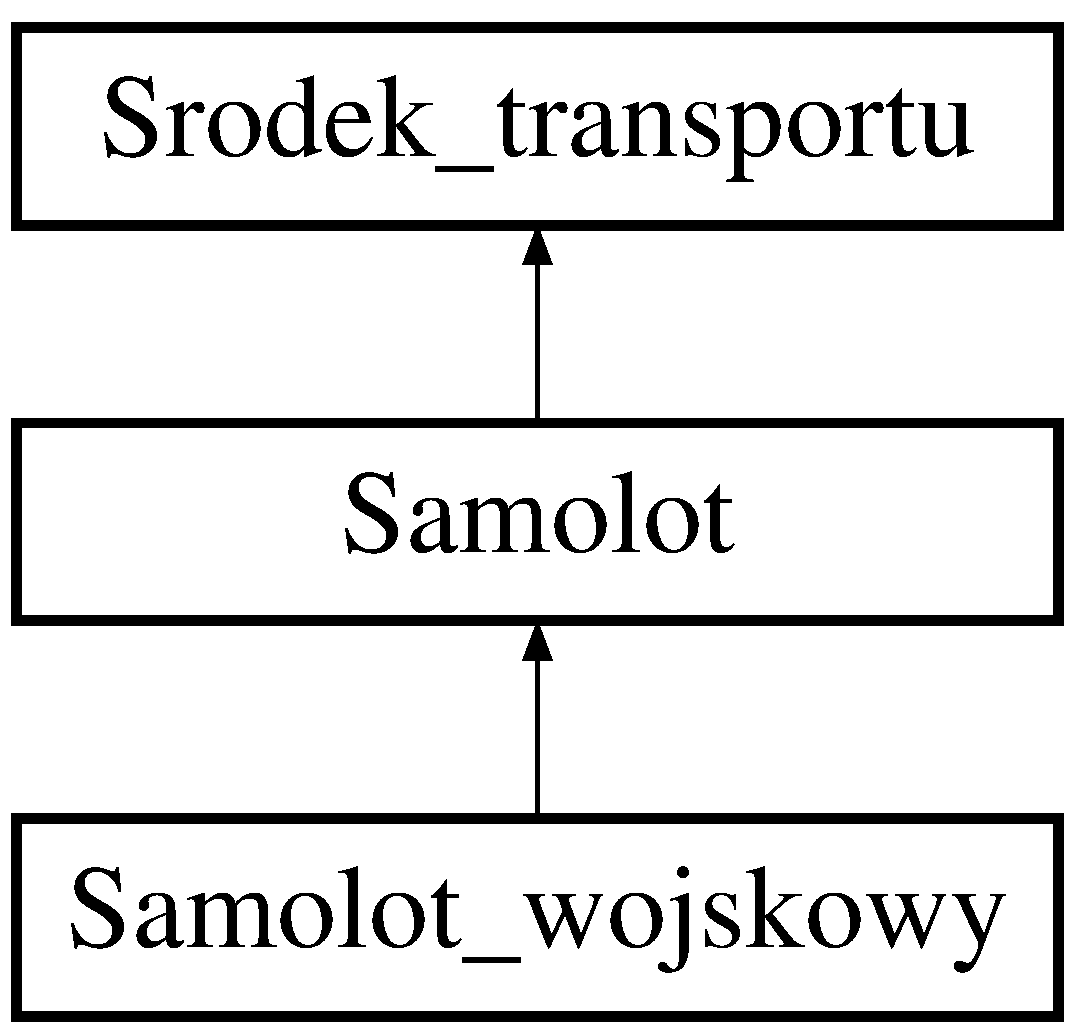
\includegraphics[height=3.000000cm]{class_samolot__wojskowy}
\end{center}
\end{figure}
\subsection*{Metody publiczne}
\begin{DoxyCompactItemize}
\item 
{\bf Samolot\+\_\+wojskowy} ()
\begin{DoxyCompactList}\small\item\em konstruktor domyslny \end{DoxyCompactList}\item 
{\bf Samolot\+\_\+wojskowy} (int miejsca, int ilosc\+\_\+osob, float max\+\_\+wys)
\begin{DoxyCompactList}\small\item\em konstruktor z parametrami \end{DoxyCompactList}\item 
{\bf $\sim$\+Samolot\+\_\+wojskowy} ()
\begin{DoxyCompactList}\small\item\em destruktor \end{DoxyCompactList}\item 
virtual void {\bf zapisz\+\_\+samolot\+\_\+wojskowy} (string nazwa)
\begin{DoxyCompactList}\small\item\em funkcja zapisu do pliku zmiennych z klasy samolot\+\_\+wojskowy \end{DoxyCompactList}\item 
virtual void {\bf wczytaj\+\_\+samolot\+\_\+wojskowy} (string nazwa)
\begin{DoxyCompactList}\small\item\em funkcja odczytu z pliku zmiennych z klasy samolot\+\_\+wojskowy \end{DoxyCompactList}\item 
void {\bf wypisz\+\_\+stan} ()
\begin{DoxyCompactList}\small\item\em funkcja wypisujaca stan samolotu wojskowego \end{DoxyCompactList}\item 
void {\bf ustaw\+\_\+domyslne} ()
\begin{DoxyCompactList}\small\item\em funkcja ustawiajaca domyslne parametry samolotu wojskowego \end{DoxyCompactList}\end{DoxyCompactItemize}
\subsection*{Atrybuty chronione}
\begin{DoxyCompactItemize}
\item 
int {\bf ilosc\+\_\+broni}
\begin{DoxyCompactList}\small\item\em zmienna przechowujaca ilosc broni \end{DoxyCompactList}\end{DoxyCompactItemize}
\subsection*{Przyjaciele}
\begin{DoxyCompactItemize}
\item 
ostream \& {\bf operator$<$$<$} (ostream \&out, {\bf Samolot\+\_\+wojskowy} \&samolot\+\_\+wojskowy)
\begin{DoxyCompactList}\small\item\em Operator strumieniowy $<$$<$. \end{DoxyCompactList}\item 
istream \& {\bf operator$>$$>$} (istream \&s, {\bf Samolot\+\_\+wojskowy} \&samolot\+\_\+wojskowy)
\begin{DoxyCompactList}\small\item\em Operator strumieniowy $>$$>$ \end{DoxyCompactList}\end{DoxyCompactItemize}
\subsection*{Dodatkowe Dziedziczone Składowe}


\subsection{Opis szczegółowy}
Klasa \doxyref{Samolot\+\_\+wojskowy}{str.}{class_samolot__wojskowy}, dziedziczy po klasie \doxyref{Samolot}{str.}{class_samolot}. 

\subsection{Dokumentacja konstruktora i destruktora}
\index{Samolot\+\_\+wojskowy@{Samolot\+\_\+wojskowy}!Samolot\+\_\+wojskowy@{Samolot\+\_\+wojskowy}}
\index{Samolot\+\_\+wojskowy@{Samolot\+\_\+wojskowy}!Samolot\+\_\+wojskowy@{Samolot\+\_\+wojskowy}}
\subsubsection[{Samolot\+\_\+wojskowy()}]{\setlength{\rightskip}{0pt plus 5cm}Samolot\+\_\+wojskowy\+::\+Samolot\+\_\+wojskowy (
\begin{DoxyParamCaption}
{}
\end{DoxyParamCaption}
)}\label{class_samolot__wojskowy_a886087627b6a64435f437bd32045d150}


konstruktor domyslny 

\index{Samolot\+\_\+wojskowy@{Samolot\+\_\+wojskowy}!Samolot\+\_\+wojskowy@{Samolot\+\_\+wojskowy}}
\index{Samolot\+\_\+wojskowy@{Samolot\+\_\+wojskowy}!Samolot\+\_\+wojskowy@{Samolot\+\_\+wojskowy}}
\subsubsection[{Samolot\+\_\+wojskowy(int miejsca, int ilosc\+\_\+osob, float max\+\_\+wys)}]{\setlength{\rightskip}{0pt plus 5cm}Samolot\+\_\+wojskowy\+::\+Samolot\+\_\+wojskowy (
\begin{DoxyParamCaption}
\item[{int}]{miejsca, }
\item[{int}]{ilosc\+\_\+osob, }
\item[{float}]{max\+\_\+wys}
\end{DoxyParamCaption}
)}\label{class_samolot__wojskowy_ade2a6e873fbfc9b2800bfdab873a4f79}


konstruktor z parametrami 

Umozliwia ustawienie ilosci miejsc, ilosci pasazerow i maksymalna wysokosc 
\begin{DoxyParams}{Parametry}
{\em miejsca} & to ilosc miejsc w samolocie \\
\hline
{\em ilosc\+\_\+osob} & jest liczba pasazerow \\
\hline
{\em max\+\_\+wys} & jest maksymalna wysokoscia lotu \\
\hline
\end{DoxyParams}
\index{Samolot\+\_\+wojskowy@{Samolot\+\_\+wojskowy}!````~Samolot\+\_\+wojskowy@{$\sim$\+Samolot\+\_\+wojskowy}}
\index{````~Samolot\+\_\+wojskowy@{$\sim$\+Samolot\+\_\+wojskowy}!Samolot\+\_\+wojskowy@{Samolot\+\_\+wojskowy}}
\subsubsection[{$\sim$\+Samolot\+\_\+wojskowy()}]{\setlength{\rightskip}{0pt plus 5cm}Samolot\+\_\+wojskowy\+::$\sim$\+Samolot\+\_\+wojskowy (
\begin{DoxyParamCaption}
{}
\end{DoxyParamCaption}
)}\label{class_samolot__wojskowy_aa6be8184e84e064c05fd8e1b8faa996e}


destruktor 



\subsection{Dokumentacja funkcji składowych}
\index{Samolot\+\_\+wojskowy@{Samolot\+\_\+wojskowy}!ustaw\+\_\+domyslne@{ustaw\+\_\+domyslne}}
\index{ustaw\+\_\+domyslne@{ustaw\+\_\+domyslne}!Samolot\+\_\+wojskowy@{Samolot\+\_\+wojskowy}}
\subsubsection[{ustaw\+\_\+domyslne()}]{\setlength{\rightskip}{0pt plus 5cm}void Samolot\+\_\+wojskowy\+::ustaw\+\_\+domyslne (
\begin{DoxyParamCaption}
{}
\end{DoxyParamCaption}
)\hspace{0.3cm}{\ttfamily [virtual]}}\label{class_samolot__wojskowy_ac5d8f5a08e9c2edfea01130d21ccf326}


funkcja ustawiajaca domyslne parametry samolotu wojskowego 



Reimplementowana z {\bf Samolot} \doxyref{}{str.}{class_samolot_a84b8eb2a9ac41911e311122973e8879f}.

\index{Samolot\+\_\+wojskowy@{Samolot\+\_\+wojskowy}!wczytaj\+\_\+samolot\+\_\+wojskowy@{wczytaj\+\_\+samolot\+\_\+wojskowy}}
\index{wczytaj\+\_\+samolot\+\_\+wojskowy@{wczytaj\+\_\+samolot\+\_\+wojskowy}!Samolot\+\_\+wojskowy@{Samolot\+\_\+wojskowy}}
\subsubsection[{wczytaj\+\_\+samolot\+\_\+wojskowy(string nazwa)}]{\setlength{\rightskip}{0pt plus 5cm}void Samolot\+\_\+wojskowy\+::wczytaj\+\_\+samolot\+\_\+wojskowy (
\begin{DoxyParamCaption}
\item[{string}]{nazwa}
\end{DoxyParamCaption}
)\hspace{0.3cm}{\ttfamily [virtual]}}\label{class_samolot__wojskowy_a3e4db07ff7f911a33a381c36e9a8af0b}


funkcja odczytu z pliku zmiennych z klasy samolot\+\_\+wojskowy 


\begin{DoxyParams}{Parametry}
{\em nazwa} & to nazwa pliku txt \\
\hline
\end{DoxyParams}
\index{Samolot\+\_\+wojskowy@{Samolot\+\_\+wojskowy}!wypisz\+\_\+stan@{wypisz\+\_\+stan}}
\index{wypisz\+\_\+stan@{wypisz\+\_\+stan}!Samolot\+\_\+wojskowy@{Samolot\+\_\+wojskowy}}
\subsubsection[{wypisz\+\_\+stan()}]{\setlength{\rightskip}{0pt plus 5cm}void Samolot\+\_\+wojskowy\+::wypisz\+\_\+stan (
\begin{DoxyParamCaption}
{}
\end{DoxyParamCaption}
)\hspace{0.3cm}{\ttfamily [virtual]}}\label{class_samolot__wojskowy_ae8670079824c05a6bbf6ba85ce13e17d}


funkcja wypisujaca stan samolotu wojskowego 



Reimplementowana z {\bf Samolot} \doxyref{}{str.}{class_samolot_a07e6de963f10b5cf7352967e736f6daa}.

\index{Samolot\+\_\+wojskowy@{Samolot\+\_\+wojskowy}!zapisz\+\_\+samolot\+\_\+wojskowy@{zapisz\+\_\+samolot\+\_\+wojskowy}}
\index{zapisz\+\_\+samolot\+\_\+wojskowy@{zapisz\+\_\+samolot\+\_\+wojskowy}!Samolot\+\_\+wojskowy@{Samolot\+\_\+wojskowy}}
\subsubsection[{zapisz\+\_\+samolot\+\_\+wojskowy(string nazwa)}]{\setlength{\rightskip}{0pt plus 5cm}void Samolot\+\_\+wojskowy\+::zapisz\+\_\+samolot\+\_\+wojskowy (
\begin{DoxyParamCaption}
\item[{string}]{nazwa}
\end{DoxyParamCaption}
)\hspace{0.3cm}{\ttfamily [virtual]}}\label{class_samolot__wojskowy_a289bd9e9c2ac172b2334ec41f1bc8d19}


funkcja zapisu do pliku zmiennych z klasy samolot\+\_\+wojskowy 


\begin{DoxyParams}{Parametry}
{\em nazwa} & to nazwa pliku txt \\
\hline
\end{DoxyParams}


\subsection{Dokumentacja przyjaciół i funkcji związanych}
\index{Samolot\+\_\+wojskowy@{Samolot\+\_\+wojskowy}!operator$<$$<$@{operator$<$$<$}}
\index{operator$<$$<$@{operator$<$$<$}!Samolot\+\_\+wojskowy@{Samolot\+\_\+wojskowy}}
\subsubsection[{operator$<$$<$}]{\setlength{\rightskip}{0pt plus 5cm}ostream\& operator$<$$<$ (
\begin{DoxyParamCaption}
\item[{ostream \&}]{out, }
\item[{{\bf Samolot\+\_\+wojskowy} \&}]{samolot\+\_\+wojskowy}
\end{DoxyParamCaption}
)\hspace{0.3cm}{\ttfamily [friend]}}\label{class_samolot__wojskowy_a1d0842843c197c48818fe3c3ddf41e8f}


Operator strumieniowy $<$$<$. 

\index{Samolot\+\_\+wojskowy@{Samolot\+\_\+wojskowy}!operator$>$$>$@{operator$>$$>$}}
\index{operator$>$$>$@{operator$>$$>$}!Samolot\+\_\+wojskowy@{Samolot\+\_\+wojskowy}}
\subsubsection[{operator$>$$>$}]{\setlength{\rightskip}{0pt plus 5cm}istream\& operator$>$$>$ (
\begin{DoxyParamCaption}
\item[{istream \&}]{s, }
\item[{{\bf Samolot\+\_\+wojskowy} \&}]{samolot\+\_\+wojskowy}
\end{DoxyParamCaption}
)\hspace{0.3cm}{\ttfamily [friend]}}\label{class_samolot__wojskowy_a703149017c7177b20bf4d47765ba7e58}


Operator strumieniowy $>$$>$ 



\subsection{Dokumentacja atrybutów składowych}
\index{Samolot\+\_\+wojskowy@{Samolot\+\_\+wojskowy}!ilosc\+\_\+broni@{ilosc\+\_\+broni}}
\index{ilosc\+\_\+broni@{ilosc\+\_\+broni}!Samolot\+\_\+wojskowy@{Samolot\+\_\+wojskowy}}
\subsubsection[{ilosc\+\_\+broni}]{\setlength{\rightskip}{0pt plus 5cm}int Samolot\+\_\+wojskowy\+::ilosc\+\_\+broni\hspace{0.3cm}{\ttfamily [protected]}}\label{class_samolot__wojskowy_a149e94bdc74aca4a9c2c04996a32d855}


zmienna przechowujaca ilosc broni 



Dokumentacja dla tej klasy została wygenerowana z plików\+:\begin{DoxyCompactItemize}
\item 
{\bf samolot\+\_\+wojskowy.\+h}\item 
{\bf samolot\+\_\+wojskowy.\+cpp}\end{DoxyCompactItemize}

\section{Dokumentacja klasy Srodek\+\_\+transportu}
\label{class_srodek__transportu}\index{Srodek\+\_\+transportu@{Srodek\+\_\+transportu}}


Klasa abstrakcyjna \doxyref{Srodek\+\_\+transportu}{str.}{class_srodek__transportu}.  




{\ttfamily \#include $<$srodek\+\_\+transportu.\+h$>$}

Diagram dziedziczenia dla Srodek\+\_\+transportu\begin{figure}[H]
\begin{center}
\leavevmode
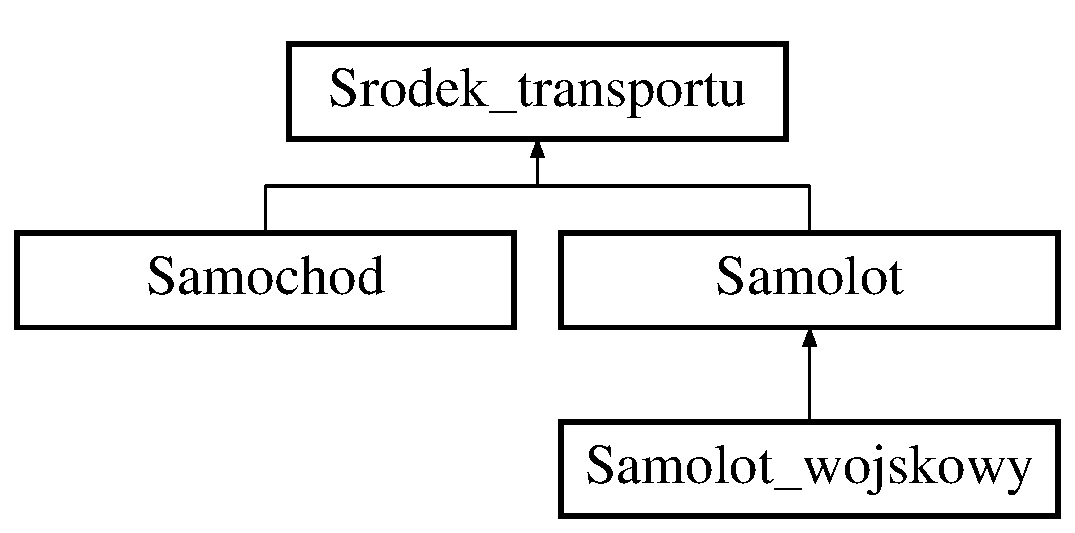
\includegraphics[height=3.000000cm]{class_srodek__transportu}
\end{center}
\end{figure}
\subsection*{Metody publiczne}
\begin{DoxyCompactItemize}
\item 
{\bf Srodek\+\_\+transportu} ()
\begin{DoxyCompactList}\small\item\em Kontruktor domy�lny. \end{DoxyCompactList}\item 
virtual {\bf $\sim$\+Srodek\+\_\+transportu} ()
\begin{DoxyCompactList}\small\item\em Destruktor wirtualny. \end{DoxyCompactList}\item 
void {\bf zapisz\+\_\+srodek} (string nazwa)
\begin{DoxyCompactList}\small\item\em funkcja zapisu do pliku zmiennych z klasy srodek\+\_\+transportu \end{DoxyCompactList}\item 
void {\bf wczytaj\+\_\+srodek} (string nazwa)
\begin{DoxyCompactList}\small\item\em funkcja odczytu z pliku zmiennych z klasy srodek\+\_\+transportu \end{DoxyCompactList}\item 
virtual void {\bf wypisz\+\_\+stan} ()=0
\begin{DoxyCompactList}\small\item\em metoda wirtualna wypisywania stanu \end{DoxyCompactList}\item 
virtual void {\bf ustaw\+\_\+domyslne} ()=0
\begin{DoxyCompactList}\small\item\em metoda wirtualna ustawiajaca domyslne dane \end{DoxyCompactList}\end{DoxyCompactItemize}
\subsection*{Atrybuty chronione}
\begin{DoxyCompactItemize}
\item 
int {\bf ilosc\+\_\+miejsc}
\begin{DoxyCompactList}\small\item\em $<$zmienna przechowujaca ilosc miejsc w srodku transportu \end{DoxyCompactList}\item 
int {\bf numer}
\item 
vector$<$ {\bf Pasazerowie} $>$ {\bf wektor\+\_\+pasazerow}
\begin{DoxyCompactList}\small\item\em wektor przechowujacy pasazerow samolotu \end{DoxyCompactList}\end{DoxyCompactItemize}
\subsection*{Przyjaciele}
\begin{DoxyCompactItemize}
\item 
std\+::ostream \& {\bf operator$<$$<$} (std\+::ostream \&s, {\bf Srodek\+\_\+transportu} \&srodek\+\_\+transportu)
\begin{DoxyCompactList}\small\item\em Operator strumieniowy $<$$<$. \end{DoxyCompactList}\item 
std\+::istream \& {\bf operator$>$$>$} (std\+::istream \&s, {\bf Srodek\+\_\+transportu} \&srodek\+\_\+transportu)
\begin{DoxyCompactList}\small\item\em Operator strumieniowy $>$$>$ \end{DoxyCompactList}\end{DoxyCompactItemize}


\subsection{Opis szczegółowy}
Klasa abstrakcyjna \doxyref{Srodek\+\_\+transportu}{str.}{class_srodek__transportu}. 

\subsection{Dokumentacja konstruktora i destruktora}
\index{Srodek\+\_\+transportu@{Srodek\+\_\+transportu}!Srodek\+\_\+transportu@{Srodek\+\_\+transportu}}
\index{Srodek\+\_\+transportu@{Srodek\+\_\+transportu}!Srodek\+\_\+transportu@{Srodek\+\_\+transportu}}
\subsubsection[{Srodek\+\_\+transportu()}]{\setlength{\rightskip}{0pt plus 5cm}Srodek\+\_\+transportu\+::\+Srodek\+\_\+transportu (
\begin{DoxyParamCaption}
{}
\end{DoxyParamCaption}
)}\label{class_srodek__transportu_a77b861f9178c4730afdf7491cc3d2d31}


Kontruktor domy�lny. 

\index{Srodek\+\_\+transportu@{Srodek\+\_\+transportu}!````~Srodek\+\_\+transportu@{$\sim$\+Srodek\+\_\+transportu}}
\index{````~Srodek\+\_\+transportu@{$\sim$\+Srodek\+\_\+transportu}!Srodek\+\_\+transportu@{Srodek\+\_\+transportu}}
\subsubsection[{$\sim$\+Srodek\+\_\+transportu()}]{\setlength{\rightskip}{0pt plus 5cm}Srodek\+\_\+transportu\+::$\sim$\+Srodek\+\_\+transportu (
\begin{DoxyParamCaption}
{}
\end{DoxyParamCaption}
)\hspace{0.3cm}{\ttfamily [virtual]}}\label{class_srodek__transportu_a14765161cda06789c3261e9ef7e3f639}


Destruktor wirtualny. 



\subsection{Dokumentacja funkcji składowych}
\index{Srodek\+\_\+transportu@{Srodek\+\_\+transportu}!ustaw\+\_\+domyslne@{ustaw\+\_\+domyslne}}
\index{ustaw\+\_\+domyslne@{ustaw\+\_\+domyslne}!Srodek\+\_\+transportu@{Srodek\+\_\+transportu}}
\subsubsection[{ustaw\+\_\+domyslne()=0}]{\setlength{\rightskip}{0pt plus 5cm}virtual void Srodek\+\_\+transportu\+::ustaw\+\_\+domyslne (
\begin{DoxyParamCaption}
{}
\end{DoxyParamCaption}
)\hspace{0.3cm}{\ttfamily [pure virtual]}}\label{class_srodek__transportu_a001cdf92b562557afa60257d174d524b}


metoda wirtualna ustawiajaca domyslne dane 



Implementowany w {\bf Samolot} \doxyref{}{str.}{class_samolot_a84b8eb2a9ac41911e311122973e8879f}, {\bf Samolot\+\_\+wojskowy} \doxyref{}{str.}{class_samolot__wojskowy_ac5d8f5a08e9c2edfea01130d21ccf326} i {\bf Samochod} \doxyref{}{str.}{class_samochod_affb67e0cc339a6fe027a82703dc4c0e9}.

\index{Srodek\+\_\+transportu@{Srodek\+\_\+transportu}!wczytaj\+\_\+srodek@{wczytaj\+\_\+srodek}}
\index{wczytaj\+\_\+srodek@{wczytaj\+\_\+srodek}!Srodek\+\_\+transportu@{Srodek\+\_\+transportu}}
\subsubsection[{wczytaj\+\_\+srodek(string nazwa)}]{\setlength{\rightskip}{0pt plus 5cm}void Srodek\+\_\+transportu\+::wczytaj\+\_\+srodek (
\begin{DoxyParamCaption}
\item[{string}]{nazwa}
\end{DoxyParamCaption}
)}\label{class_srodek__transportu_a0f8007748ab99f18d2bb6b1cb3f684ab}


funkcja odczytu z pliku zmiennych z klasy srodek\+\_\+transportu 


\begin{DoxyParams}{Parametry}
{\em nazwa} & to nazwa pliku txt \\
\hline
\end{DoxyParams}
\index{Srodek\+\_\+transportu@{Srodek\+\_\+transportu}!wypisz\+\_\+stan@{wypisz\+\_\+stan}}
\index{wypisz\+\_\+stan@{wypisz\+\_\+stan}!Srodek\+\_\+transportu@{Srodek\+\_\+transportu}}
\subsubsection[{wypisz\+\_\+stan()=0}]{\setlength{\rightskip}{0pt plus 5cm}virtual void Srodek\+\_\+transportu\+::wypisz\+\_\+stan (
\begin{DoxyParamCaption}
{}
\end{DoxyParamCaption}
)\hspace{0.3cm}{\ttfamily [pure virtual]}}\label{class_srodek__transportu_aed5cfb50e521972271e878d947d7cc5c}


metoda wirtualna wypisywania stanu 



Implementowany w {\bf Samolot} \doxyref{}{str.}{class_samolot_a07e6de963f10b5cf7352967e736f6daa}, {\bf Samolot\+\_\+wojskowy} \doxyref{}{str.}{class_samolot__wojskowy_ae8670079824c05a6bbf6ba85ce13e17d} i {\bf Samochod} \doxyref{}{str.}{class_samochod_a45373f78f0764700a4eed0b34c300915}.

\index{Srodek\+\_\+transportu@{Srodek\+\_\+transportu}!zapisz\+\_\+srodek@{zapisz\+\_\+srodek}}
\index{zapisz\+\_\+srodek@{zapisz\+\_\+srodek}!Srodek\+\_\+transportu@{Srodek\+\_\+transportu}}
\subsubsection[{zapisz\+\_\+srodek(string nazwa)}]{\setlength{\rightskip}{0pt plus 5cm}void Srodek\+\_\+transportu\+::zapisz\+\_\+srodek (
\begin{DoxyParamCaption}
\item[{string}]{nazwa}
\end{DoxyParamCaption}
)}\label{class_srodek__transportu_a6a595208ccebdf6b64eb7be7ea4f0826}


funkcja zapisu do pliku zmiennych z klasy srodek\+\_\+transportu 


\begin{DoxyParams}{Parametry}
{\em nazwa} & to nazwa pliku txt \\
\hline
\end{DoxyParams}


\subsection{Dokumentacja przyjaciół i funkcji związanych}
\index{Srodek\+\_\+transportu@{Srodek\+\_\+transportu}!operator$<$$<$@{operator$<$$<$}}
\index{operator$<$$<$@{operator$<$$<$}!Srodek\+\_\+transportu@{Srodek\+\_\+transportu}}
\subsubsection[{operator$<$$<$}]{\setlength{\rightskip}{0pt plus 5cm}std\+::ostream\& operator$<$$<$ (
\begin{DoxyParamCaption}
\item[{std\+::ostream \&}]{s, }
\item[{{\bf Srodek\+\_\+transportu} \&}]{srodek\+\_\+transportu}
\end{DoxyParamCaption}
)\hspace{0.3cm}{\ttfamily [friend]}}\label{class_srodek__transportu_a03f7d6e2b1da2f66e09b3ee3bb086e1c}


Operator strumieniowy $<$$<$. 

\index{Srodek\+\_\+transportu@{Srodek\+\_\+transportu}!operator$>$$>$@{operator$>$$>$}}
\index{operator$>$$>$@{operator$>$$>$}!Srodek\+\_\+transportu@{Srodek\+\_\+transportu}}
\subsubsection[{operator$>$$>$}]{\setlength{\rightskip}{0pt plus 5cm}std\+::istream\& operator$>$$>$ (
\begin{DoxyParamCaption}
\item[{std\+::istream \&}]{s, }
\item[{{\bf Srodek\+\_\+transportu} \&}]{srodek\+\_\+transportu}
\end{DoxyParamCaption}
)\hspace{0.3cm}{\ttfamily [friend]}}\label{class_srodek__transportu_a0d7ca7f7dd615d2fab10c64f9155a428}


Operator strumieniowy $>$$>$ 



\subsection{Dokumentacja atrybutów składowych}
\index{Srodek\+\_\+transportu@{Srodek\+\_\+transportu}!ilosc\+\_\+miejsc@{ilosc\+\_\+miejsc}}
\index{ilosc\+\_\+miejsc@{ilosc\+\_\+miejsc}!Srodek\+\_\+transportu@{Srodek\+\_\+transportu}}
\subsubsection[{ilosc\+\_\+miejsc}]{\setlength{\rightskip}{0pt plus 5cm}int Srodek\+\_\+transportu\+::ilosc\+\_\+miejsc\hspace{0.3cm}{\ttfamily [protected]}}\label{class_srodek__transportu_abc206dbf871266b8a818b3338be71e81}


$<$zmienna przechowujaca ilosc miejsc w srodku transportu 

zmienna przechowujaca numer srodku transportu \index{Srodek\+\_\+transportu@{Srodek\+\_\+transportu}!numer@{numer}}
\index{numer@{numer}!Srodek\+\_\+transportu@{Srodek\+\_\+transportu}}
\subsubsection[{numer}]{\setlength{\rightskip}{0pt plus 5cm}int Srodek\+\_\+transportu\+::numer\hspace{0.3cm}{\ttfamily [protected]}}\label{class_srodek__transportu_aff822a566bc2403d4d99a9155771f8bc}
\index{Srodek\+\_\+transportu@{Srodek\+\_\+transportu}!wektor\+\_\+pasazerow@{wektor\+\_\+pasazerow}}
\index{wektor\+\_\+pasazerow@{wektor\+\_\+pasazerow}!Srodek\+\_\+transportu@{Srodek\+\_\+transportu}}
\subsubsection[{wektor\+\_\+pasazerow}]{\setlength{\rightskip}{0pt plus 5cm}vector$<${\bf Pasazerowie}$>$ Srodek\+\_\+transportu\+::wektor\+\_\+pasazerow\hspace{0.3cm}{\ttfamily [protected]}}\label{class_srodek__transportu_ae54b5f56778df51d0efd28bddebed26e}


wektor przechowujacy pasazerow samolotu 



Dokumentacja dla tej klasy została wygenerowana z plików\+:\begin{DoxyCompactItemize}
\item 
{\bf srodek\+\_\+transportu.\+h}\item 
{\bf srodek\+\_\+transportu.\+cpp}\end{DoxyCompactItemize}

\section{Dokumentacja klasy Zaloga}
\label{class_zaloga}\index{Zaloga@{Zaloga}}


Klasa \doxyref{Zaloga}{str.}{class_zaloga}.  




{\ttfamily \#include $<$zaloga.\+h$>$}

\subsection*{Metody publiczne}
\begin{DoxyCompactItemize}
\item 
{\bf Zaloga} ()
\begin{DoxyCompactList}\small\item\em konstruktor domyslny \end{DoxyCompactList}\item 
{\bf $\sim$\+Zaloga} ()
\begin{DoxyCompactList}\small\item\em destruktor \end{DoxyCompactList}\item 
void {\bf zmienid} (int noweid)
\begin{DoxyCompactList}\small\item\em metoda umozliwiajaca zmiane id \end{DoxyCompactList}\item 
bool {\bf operator==} (const {\bf Zaloga} \&zaloga1)
\begin{DoxyCompactList}\small\item\em przeciazony operator == \end{DoxyCompactList}\end{DoxyCompactItemize}
\subsection*{Przyjaciele}
\begin{DoxyCompactItemize}
\item 
ostream \& {\bf operator$<$$<$} (ostream \&out, {\bf Zaloga} \&zaloga)
\begin{DoxyCompactList}\small\item\em Operator strumieniowy $<$$<$. \end{DoxyCompactList}\item 
istream \& {\bf operator$>$$>$} (istream \&s, {\bf Zaloga} \&zaloga)
\begin{DoxyCompactList}\small\item\em Operator strumieniowy $>$$>$ \end{DoxyCompactList}\end{DoxyCompactItemize}


\subsection{Opis szczegółowy}
Klasa \doxyref{Zaloga}{str.}{class_zaloga}. 

\subsection{Dokumentacja konstruktora i destruktora}
\index{Zaloga@{Zaloga}!Zaloga@{Zaloga}}
\index{Zaloga@{Zaloga}!Zaloga@{Zaloga}}
\subsubsection[{Zaloga()}]{\setlength{\rightskip}{0pt plus 5cm}Zaloga\+::\+Zaloga (
\begin{DoxyParamCaption}
{}
\end{DoxyParamCaption}
)}\label{class_zaloga_ae4f1ed441b1d95e916c87622564acc03}


konstruktor domyslny 

\index{Zaloga@{Zaloga}!````~Zaloga@{$\sim$\+Zaloga}}
\index{````~Zaloga@{$\sim$\+Zaloga}!Zaloga@{Zaloga}}
\subsubsection[{$\sim$\+Zaloga()}]{\setlength{\rightskip}{0pt plus 5cm}Zaloga\+::$\sim$\+Zaloga (
\begin{DoxyParamCaption}
{}
\end{DoxyParamCaption}
)}\label{class_zaloga_a0b8f946de0ee9eda41b8a11b2678ca74}


destruktor 



\subsection{Dokumentacja funkcji składowych}
\index{Zaloga@{Zaloga}!operator==@{operator==}}
\index{operator==@{operator==}!Zaloga@{Zaloga}}
\subsubsection[{operator==(const Zaloga \&zaloga1)}]{\setlength{\rightskip}{0pt plus 5cm}bool Zaloga\+::operator== (
\begin{DoxyParamCaption}
\item[{const {\bf Zaloga} \&}]{zaloga1}
\end{DoxyParamCaption}
)}\label{class_zaloga_a9a91cc95c947e41789310dd0cc383ddb}


przeciazony operator == 

\index{Zaloga@{Zaloga}!zmienid@{zmienid}}
\index{zmienid@{zmienid}!Zaloga@{Zaloga}}
\subsubsection[{zmienid(int noweid)}]{\setlength{\rightskip}{0pt plus 5cm}void Zaloga\+::zmienid (
\begin{DoxyParamCaption}
\item[{int}]{noweid}
\end{DoxyParamCaption}
)}\label{class_zaloga_acde30ea6bbf193d9e57fc38817b50939}


metoda umozliwiajaca zmiane id 


\begin{DoxyParams}{Parametry}
{\em nowe} & id pilota \\
\hline
\end{DoxyParams}
\begin{DoxyReturn}{Zwraca}
nic nie zwraca 
\end{DoxyReturn}


\subsection{Dokumentacja przyjaciół i funkcji związanych}
\index{Zaloga@{Zaloga}!operator$<$$<$@{operator$<$$<$}}
\index{operator$<$$<$@{operator$<$$<$}!Zaloga@{Zaloga}}
\subsubsection[{operator$<$$<$}]{\setlength{\rightskip}{0pt plus 5cm}ostream\& operator$<$$<$ (
\begin{DoxyParamCaption}
\item[{ostream \&}]{out, }
\item[{{\bf Zaloga} \&}]{zaloga}
\end{DoxyParamCaption}
)\hspace{0.3cm}{\ttfamily [friend]}}\label{class_zaloga_a8e9e212da88b200af0a25ea0daadb4c5}


Operator strumieniowy $<$$<$. 

\index{Zaloga@{Zaloga}!operator$>$$>$@{operator$>$$>$}}
\index{operator$>$$>$@{operator$>$$>$}!Zaloga@{Zaloga}}
\subsubsection[{operator$>$$>$}]{\setlength{\rightskip}{0pt plus 5cm}istream\& operator$>$$>$ (
\begin{DoxyParamCaption}
\item[{istream \&}]{s, }
\item[{{\bf Zaloga} \&}]{zaloga}
\end{DoxyParamCaption}
)\hspace{0.3cm}{\ttfamily [friend]}}\label{class_zaloga_af1a931d5a0f1a0d95c73c35cd085858d}


Operator strumieniowy $>$$>$ 



Dokumentacja dla tej klasy została wygenerowana z plików\+:\begin{DoxyCompactItemize}
\item 
{\bf zaloga.\+h}\item 
{\bf zaloga.\+cpp}\end{DoxyCompactItemize}

\chapter{Dokumentacja plików}
\section{Dokumentacja pliku dane\+\_\+samolotu.\+cpp}
\label{dane__samolotu_8cpp}\index{dane\+\_\+samolotu.\+cpp@{dane\+\_\+samolotu.\+cpp}}
{\ttfamily \#include $<$iostream$>$}\\*
{\ttfamily \#include $<$string$>$}\\*
{\ttfamily \#include $<$fstream$>$}\\*
{\ttfamily \#include \char`\"{}dane\+\_\+samolotu.\+h\char`\"{}}\\*
\subsection*{Funkcje}
\begin{DoxyCompactItemize}
\item 
ostream \& {\bf operator$<$$<$} (ostream \&out, {\bf Dane\+Samolotu} \&dane)
\item 
istream \& {\bf operator$>$$>$} (istream \&s, {\bf Dane\+Samolotu} \&dane)
\end{DoxyCompactItemize}


\subsection{Dokumentacja funkcji}
\index{dane\+\_\+samolotu.\+cpp@{dane\+\_\+samolotu.\+cpp}!operator$<$$<$@{operator$<$$<$}}
\index{operator$<$$<$@{operator$<$$<$}!dane\+\_\+samolotu.\+cpp@{dane\+\_\+samolotu.\+cpp}}
\subsubsection[{operator$<$$<$(ostream \&out, Dane\+Samolotu \&dane)}]{\setlength{\rightskip}{0pt plus 5cm}ostream\& operator$<$$<$ (
\begin{DoxyParamCaption}
\item[{ostream \&}]{out, }
\item[{{\bf Dane\+Samolotu} \&}]{dane}
\end{DoxyParamCaption}
)}\label{dane__samolotu_8cpp_aaaf6a3db89522d407cf92091a98c2e80}
\index{dane\+\_\+samolotu.\+cpp@{dane\+\_\+samolotu.\+cpp}!operator$>$$>$@{operator$>$$>$}}
\index{operator$>$$>$@{operator$>$$>$}!dane\+\_\+samolotu.\+cpp@{dane\+\_\+samolotu.\+cpp}}
\subsubsection[{operator$>$$>$(istream \&s, Dane\+Samolotu \&dane)}]{\setlength{\rightskip}{0pt plus 5cm}istream\& operator$>$$>$ (
\begin{DoxyParamCaption}
\item[{istream \&}]{s, }
\item[{{\bf Dane\+Samolotu} \&}]{dane}
\end{DoxyParamCaption}
)}\label{dane__samolotu_8cpp_ae1a66a9e4246344008e3874910e3045d}

\section{Dokumentacja pliku dane\+\_\+samolotu.\+h}
\label{dane__samolotu_8h}\index{dane\+\_\+samolotu.\+h@{dane\+\_\+samolotu.\+h}}
{\ttfamily \#include $<$string$>$}\\*
{\ttfamily \#include $<$iostream$>$}\\*
{\ttfamily \#include $<$fstream$>$}\\*
\subsection*{Komponenty}
\begin{DoxyCompactItemize}
\item 
class {\bf Dane\+Samolotu}
\begin{DoxyCompactList}\small\item\em klasa \doxyref{Dane\+Samolotu}{str.}{class_dane_samolotu} \end{DoxyCompactList}\end{DoxyCompactItemize}

\section{Dokumentacja pliku pasazerowie.\+cpp}
\label{pasazerowie_8cpp}\index{pasazerowie.\+cpp@{pasazerowie.\+cpp}}
{\ttfamily \#include $<$iostream$>$}\\*
{\ttfamily \#include $<$string$>$}\\*
{\ttfamily \#include $<$fstream$>$}\\*
{\ttfamily \#include \char`\"{}pasazerowie.\+h\char`\"{}}\\*
\subsection*{Funkcje}
\begin{DoxyCompactItemize}
\item 
ostream \& {\bf operator$<$$<$} (ostream \&out, {\bf Pasazerowie} \&pasazerowie)
\item 
istream \& {\bf operator$>$$>$} (istream \&s, {\bf Pasazerowie} \&pasazerowie)
\end{DoxyCompactItemize}


\subsection{Dokumentacja funkcji}
\index{pasazerowie.\+cpp@{pasazerowie.\+cpp}!operator$<$$<$@{operator$<$$<$}}
\index{operator$<$$<$@{operator$<$$<$}!pasazerowie.\+cpp@{pasazerowie.\+cpp}}
\subsubsection[{operator$<$$<$(ostream \&out, Pasazerowie \&pasazerowie)}]{\setlength{\rightskip}{0pt plus 5cm}ostream\& operator$<$$<$ (
\begin{DoxyParamCaption}
\item[{ostream \&}]{out, }
\item[{{\bf Pasazerowie} \&}]{pasazerowie}
\end{DoxyParamCaption}
)}\label{pasazerowie_8cpp_a2450aa552025411d4775ec11a1d091d2}
\index{pasazerowie.\+cpp@{pasazerowie.\+cpp}!operator$>$$>$@{operator$>$$>$}}
\index{operator$>$$>$@{operator$>$$>$}!pasazerowie.\+cpp@{pasazerowie.\+cpp}}
\subsubsection[{operator$>$$>$(istream \&s, Pasazerowie \&pasazerowie)}]{\setlength{\rightskip}{0pt plus 5cm}istream\& operator$>$$>$ (
\begin{DoxyParamCaption}
\item[{istream \&}]{s, }
\item[{{\bf Pasazerowie} \&}]{pasazerowie}
\end{DoxyParamCaption}
)}\label{pasazerowie_8cpp_a42b7ff0865bca4ed3d43a45b68c7bcdd}

\section{Dokumentacja pliku pasazerowie.\+h}
\label{pasazerowie_8h}\index{pasazerowie.\+h@{pasazerowie.\+h}}
{\ttfamily \#include $<$string$>$}\\*
{\ttfamily \#include $<$iostream$>$}\\*
{\ttfamily \#include $<$fstream$>$}\\*
\subsection*{Komponenty}
\begin{DoxyCompactItemize}
\item 
class {\bf Pasazerowie}
\begin{DoxyCompactList}\small\item\em klasa \doxyref{Pasazerowie}{str.}{class_pasazerowie} \end{DoxyCompactList}\end{DoxyCompactItemize}

\section{Dokumentacja pliku program.\+cpp}
\label{program_8cpp}\index{program.\+cpp@{program.\+cpp}}
{\ttfamily \#include $<$iostream$>$}\\*
{\ttfamily \#include $<$string$>$}\\*
{\ttfamily \#include \char`\"{}srodek\+\_\+transportu.\+h\char`\"{}}\\*
{\ttfamily \#include \char`\"{}samolot.\+h\char`\"{}}\\*
{\ttfamily \#include \char`\"{}samolot\+\_\+wojskowy.\+h\char`\"{}}\\*
{\ttfamily \#include \char`\"{}samochod.\+h\char`\"{}}\\*
{\ttfamily \#include $<$vector$>$}\\*
\subsection*{Funkcje}
\begin{DoxyCompactItemize}
\item 
void {\bf testuj} ()
\item 
int {\bf main} ()
\end{DoxyCompactItemize}


\subsection{Dokumentacja funkcji}
\index{program.\+cpp@{program.\+cpp}!main@{main}}
\index{main@{main}!program.\+cpp@{program.\+cpp}}
\subsubsection[{main()}]{\setlength{\rightskip}{0pt plus 5cm}int main (
\begin{DoxyParamCaption}
{}
\end{DoxyParamCaption}
)}\label{program_8cpp_ae66f6b31b5ad750f1fe042a706a4e3d4}
\index{program.\+cpp@{program.\+cpp}!testuj@{testuj}}
\index{testuj@{testuj}!program.\+cpp@{program.\+cpp}}
\subsubsection[{testuj()}]{\setlength{\rightskip}{0pt plus 5cm}void testuj (
\begin{DoxyParamCaption}
{}
\end{DoxyParamCaption}
)}\label{program_8cpp_a50eab1c6c0da1d19bdf40e77f2433a8e}

\section{Dokumentacja pliku samochod.\+cpp}
\label{samochod_8cpp}\index{samochod.\+cpp@{samochod.\+cpp}}
{\ttfamily \#include $<$iostream$>$}\\*
{\ttfamily \#include $<$string$>$}\\*
{\ttfamily \#include $<$fstream$>$}\\*
{\ttfamily \#include \char`\"{}samochod.\+h\char`\"{}}\\*
\subsection*{Funkcje}
\begin{DoxyCompactItemize}
\item 
ostream \& {\bf operator$<$$<$} (ostream \&out, {\bf Samochod} \&samochod)
\item 
istream \& {\bf operator$>$$>$} (istream \&s, {\bf Samochod} \&samochod)
\end{DoxyCompactItemize}


\subsection{Dokumentacja funkcji}
\index{samochod.\+cpp@{samochod.\+cpp}!operator$<$$<$@{operator$<$$<$}}
\index{operator$<$$<$@{operator$<$$<$}!samochod.\+cpp@{samochod.\+cpp}}
\subsubsection[{operator$<$$<$(ostream \&out, Samochod \&samochod)}]{\setlength{\rightskip}{0pt plus 5cm}ostream\& operator$<$$<$ (
\begin{DoxyParamCaption}
\item[{ostream \&}]{out, }
\item[{{\bf Samochod} \&}]{samochod}
\end{DoxyParamCaption}
)}\label{samochod_8cpp_a48c7afb882b656c44f52e8a92c26a34b}
\index{samochod.\+cpp@{samochod.\+cpp}!operator$>$$>$@{operator$>$$>$}}
\index{operator$>$$>$@{operator$>$$>$}!samochod.\+cpp@{samochod.\+cpp}}
\subsubsection[{operator$>$$>$(istream \&s, Samochod \&samochod)}]{\setlength{\rightskip}{0pt plus 5cm}istream\& operator$>$$>$ (
\begin{DoxyParamCaption}
\item[{istream \&}]{s, }
\item[{{\bf Samochod} \&}]{samochod}
\end{DoxyParamCaption}
)}\label{samochod_8cpp_a2ee8222931a9b95803d5a280ebe8ee96}

\section{Dokumentacja pliku samochod.\+h}
\label{samochod_8h}\index{samochod.\+h@{samochod.\+h}}
{\ttfamily \#include $<$iostream$>$}\\*
{\ttfamily \#include $<$fstream$>$}\\*
{\ttfamily \#include \char`\"{}srodek\+\_\+transportu.\+h\char`\"{}}\\*
\subsection*{Komponenty}
\begin{DoxyCompactItemize}
\item 
class {\bf Samochod}
\begin{DoxyCompactList}\small\item\em Klasa \doxyref{Samochod}{str.}{class_samochod}, dziedziczy po klasie \doxyref{Srodek\+\_\+transportu}{str.}{class_srodek__transportu}. \end{DoxyCompactList}\end{DoxyCompactItemize}

\section{Dokumentacja pliku samolot.\+cpp}
\label{samolot_8cpp}\index{samolot.\+cpp@{samolot.\+cpp}}
{\ttfamily \#include $<$iostream$>$}\\*
{\ttfamily \#include $<$string$>$}\\*
{\ttfamily \#include $<$fstream$>$}\\*
{\ttfamily \#include $<$vector$>$}\\*
{\ttfamily \#include \char`\"{}samolot.\+h\char`\"{}}\\*
\subsection*{Funkcje}
\begin{DoxyCompactItemize}
\item 
ostream \& {\bf operator$<$$<$} (ostream \&out, {\bf Samolot} \&samolot)
\item 
istream \& {\bf operator$>$$>$} (istream \&s, {\bf Samolot} \&samolot)
\end{DoxyCompactItemize}


\subsection{Dokumentacja funkcji}
\index{samolot.\+cpp@{samolot.\+cpp}!operator$<$$<$@{operator$<$$<$}}
\index{operator$<$$<$@{operator$<$$<$}!samolot.\+cpp@{samolot.\+cpp}}
\subsubsection[{operator$<$$<$(ostream \&out, Samolot \&samolot)}]{\setlength{\rightskip}{0pt plus 5cm}ostream\& operator$<$$<$ (
\begin{DoxyParamCaption}
\item[{ostream \&}]{out, }
\item[{{\bf Samolot} \&}]{samolot}
\end{DoxyParamCaption}
)}\label{samolot_8cpp_a82db46739380d91ece30822283949c31}
\index{samolot.\+cpp@{samolot.\+cpp}!operator$>$$>$@{operator$>$$>$}}
\index{operator$>$$>$@{operator$>$$>$}!samolot.\+cpp@{samolot.\+cpp}}
\subsubsection[{operator$>$$>$(istream \&s, Samolot \&samolot)}]{\setlength{\rightskip}{0pt plus 5cm}istream\& operator$>$$>$ (
\begin{DoxyParamCaption}
\item[{istream \&}]{s, }
\item[{{\bf Samolot} \&}]{samolot}
\end{DoxyParamCaption}
)}\label{samolot_8cpp_a217b84d2f9887c1e78cdb41b685f6441}

\section{Dokumentacja pliku samolot.\+h}
\label{samolot_8h}\index{samolot.\+h@{samolot.\+h}}
{\ttfamily \#include $<$string$>$}\\*
{\ttfamily \#include $<$iostream$>$}\\*
{\ttfamily \#include $<$fstream$>$}\\*
{\ttfamily \#include \char`\"{}zaloga.\+h\char`\"{}}\\*
{\ttfamily \#include \char`\"{}dane\+\_\+samolotu.\+h\char`\"{}}\\*
{\ttfamily \#include \char`\"{}srodek\+\_\+transportu.\+h\char`\"{}}\\*
{\ttfamily \#include $<$vector$>$}\\*
\subsection*{Komponenty}
\begin{DoxyCompactItemize}
\item 
class {\bf Samolot}
\begin{DoxyCompactList}\small\item\em Klasa \doxyref{Samolot}{str.}{class_samolot}, dziedziczy po klasie \doxyref{Srodek\+\_\+transportu}{str.}{class_srodek__transportu}. \end{DoxyCompactList}\end{DoxyCompactItemize}

\section{Dokumentacja pliku samolot\+\_\+wojskowy.\+cpp}
\label{samolot__wojskowy_8cpp}\index{samolot\+\_\+wojskowy.\+cpp@{samolot\+\_\+wojskowy.\+cpp}}
{\ttfamily \#include $<$iostream$>$}\\*
{\ttfamily \#include $<$string$>$}\\*
{\ttfamily \#include $<$fstream$>$}\\*
{\ttfamily \#include \char`\"{}samolot\+\_\+wojskowy.\+h\char`\"{}}\\*
\subsection*{Funkcje}
\begin{DoxyCompactItemize}
\item 
ostream \& {\bf operator$<$$<$} (ostream \&out, {\bf Samolot\+\_\+wojskowy} \&samolot\+\_\+wojskowy)
\item 
istream \& {\bf operator$>$$>$} (istream \&s, {\bf Samolot\+\_\+wojskowy} \&samolot\+\_\+wojskowy)
\end{DoxyCompactItemize}


\subsection{Dokumentacja funkcji}
\index{samolot\+\_\+wojskowy.\+cpp@{samolot\+\_\+wojskowy.\+cpp}!operator$<$$<$@{operator$<$$<$}}
\index{operator$<$$<$@{operator$<$$<$}!samolot\+\_\+wojskowy.\+cpp@{samolot\+\_\+wojskowy.\+cpp}}
\subsubsection[{operator$<$$<$(ostream \&out, Samolot\+\_\+wojskowy \&samolot\+\_\+wojskowy)}]{\setlength{\rightskip}{0pt plus 5cm}ostream\& operator$<$$<$ (
\begin{DoxyParamCaption}
\item[{ostream \&}]{out, }
\item[{{\bf Samolot\+\_\+wojskowy} \&}]{samolot\+\_\+wojskowy}
\end{DoxyParamCaption}
)}\label{samolot__wojskowy_8cpp_a1d0842843c197c48818fe3c3ddf41e8f}
\index{samolot\+\_\+wojskowy.\+cpp@{samolot\+\_\+wojskowy.\+cpp}!operator$>$$>$@{operator$>$$>$}}
\index{operator$>$$>$@{operator$>$$>$}!samolot\+\_\+wojskowy.\+cpp@{samolot\+\_\+wojskowy.\+cpp}}
\subsubsection[{operator$>$$>$(istream \&s, Samolot\+\_\+wojskowy \&samolot\+\_\+wojskowy)}]{\setlength{\rightskip}{0pt plus 5cm}istream\& operator$>$$>$ (
\begin{DoxyParamCaption}
\item[{istream \&}]{s, }
\item[{{\bf Samolot\+\_\+wojskowy} \&}]{samolot\+\_\+wojskowy}
\end{DoxyParamCaption}
)}\label{samolot__wojskowy_8cpp_a703149017c7177b20bf4d47765ba7e58}

\section{Dokumentacja pliku samolot\+\_\+wojskowy.\+h}
\label{samolot__wojskowy_8h}\index{samolot\+\_\+wojskowy.\+h@{samolot\+\_\+wojskowy.\+h}}
{\ttfamily \#include $<$iostream$>$}\\*
{\ttfamily \#include $<$fstream$>$}\\*
{\ttfamily \#include \char`\"{}samolot.\+h\char`\"{}}\\*
\subsection*{Komponenty}
\begin{DoxyCompactItemize}
\item 
class {\bf Samolot\+\_\+wojskowy}
\begin{DoxyCompactList}\small\item\em Klasa \doxyref{Samolot\+\_\+wojskowy}{str.}{class_samolot__wojskowy}, dziedziczy po klasie \doxyref{Samolot}{str.}{class_samolot}. \end{DoxyCompactList}\end{DoxyCompactItemize}

\section{Dokumentacja pliku srodek\+\_\+transportu.\+cpp}
\label{srodek__transportu_8cpp}\index{srodek\+\_\+transportu.\+cpp@{srodek\+\_\+transportu.\+cpp}}
{\ttfamily \#include $<$iostream$>$}\\*
{\ttfamily \#include $<$string$>$}\\*
{\ttfamily \#include $<$fstream$>$}\\*
{\ttfamily \#include \char`\"{}srodek\+\_\+transportu.\+h\char`\"{}}\\*
\subsection*{Funkcje}
\begin{DoxyCompactItemize}
\item 
ostream \& {\bf operator$<$$<$} (ostream \&out, {\bf Srodek\+\_\+transportu} \&srodek\+\_\+transportu)
\item 
istream \& {\bf operator$>$$>$} (istream \&s, {\bf Srodek\+\_\+transportu} \&srodek\+\_\+transportu)
\end{DoxyCompactItemize}


\subsection{Dokumentacja funkcji}
\index{srodek\+\_\+transportu.\+cpp@{srodek\+\_\+transportu.\+cpp}!operator$<$$<$@{operator$<$$<$}}
\index{operator$<$$<$@{operator$<$$<$}!srodek\+\_\+transportu.\+cpp@{srodek\+\_\+transportu.\+cpp}}
\subsubsection[{operator$<$$<$(ostream \&out, Srodek\+\_\+transportu \&srodek\+\_\+transportu)}]{\setlength{\rightskip}{0pt plus 5cm}ostream\& operator$<$$<$ (
\begin{DoxyParamCaption}
\item[{ostream \&}]{out, }
\item[{{\bf Srodek\+\_\+transportu} \&}]{srodek\+\_\+transportu}
\end{DoxyParamCaption}
)}\label{srodek__transportu_8cpp_a3eca7d4984e90dea95246fbb7a04c337}
\index{srodek\+\_\+transportu.\+cpp@{srodek\+\_\+transportu.\+cpp}!operator$>$$>$@{operator$>$$>$}}
\index{operator$>$$>$@{operator$>$$>$}!srodek\+\_\+transportu.\+cpp@{srodek\+\_\+transportu.\+cpp}}
\subsubsection[{operator$>$$>$(istream \&s, Srodek\+\_\+transportu \&srodek\+\_\+transportu)}]{\setlength{\rightskip}{0pt plus 5cm}istream\& operator$>$$>$ (
\begin{DoxyParamCaption}
\item[{istream \&}]{s, }
\item[{{\bf Srodek\+\_\+transportu} \&}]{srodek\+\_\+transportu}
\end{DoxyParamCaption}
)}\label{srodek__transportu_8cpp_a73a6bb84dc14b1ebe72bacf5b976915b}

\section{Dokumentacja pliku srodek\+\_\+transportu.\+h}
\label{srodek__transportu_8h}\index{srodek\+\_\+transportu.\+h@{srodek\+\_\+transportu.\+h}}
{\ttfamily \#include $<$iostream$>$}\\*
{\ttfamily \#include $<$fstream$>$}\\*
{\ttfamily \#include $<$vector$>$}\\*
{\ttfamily \#include \char`\"{}pasazerowie.\+h\char`\"{}}\\*
\subsection*{Komponenty}
\begin{DoxyCompactItemize}
\item 
class {\bf Srodek\+\_\+transportu}
\begin{DoxyCompactList}\small\item\em Klasa abstrakcyjna \doxyref{Srodek\+\_\+transportu}{str.}{class_srodek__transportu}. \end{DoxyCompactList}\end{DoxyCompactItemize}

\section{Dokumentacja pliku zaloga.\+cpp}
\label{zaloga_8cpp}\index{zaloga.\+cpp@{zaloga.\+cpp}}
{\ttfamily \#include $<$iostream$>$}\\*
{\ttfamily \#include $<$string$>$}\\*
{\ttfamily \#include $<$fstream$>$}\\*
{\ttfamily \#include \char`\"{}zaloga.\+h\char`\"{}}\\*
\subsection*{Funkcje}
\begin{DoxyCompactItemize}
\item 
ostream \& {\bf operator$<$$<$} (ostream \&out, {\bf Zaloga} \&zaloga)
\item 
istream \& {\bf operator$>$$>$} (istream \&s, {\bf Zaloga} \&zaloga)
\end{DoxyCompactItemize}


\subsection{Dokumentacja funkcji}
\index{zaloga.\+cpp@{zaloga.\+cpp}!operator$<$$<$@{operator$<$$<$}}
\index{operator$<$$<$@{operator$<$$<$}!zaloga.\+cpp@{zaloga.\+cpp}}
\subsubsection[{operator$<$$<$(ostream \&out, Zaloga \&zaloga)}]{\setlength{\rightskip}{0pt plus 5cm}ostream\& operator$<$$<$ (
\begin{DoxyParamCaption}
\item[{ostream \&}]{out, }
\item[{{\bf Zaloga} \&}]{zaloga}
\end{DoxyParamCaption}
)}\label{zaloga_8cpp_a8e9e212da88b200af0a25ea0daadb4c5}
\index{zaloga.\+cpp@{zaloga.\+cpp}!operator$>$$>$@{operator$>$$>$}}
\index{operator$>$$>$@{operator$>$$>$}!zaloga.\+cpp@{zaloga.\+cpp}}
\subsubsection[{operator$>$$>$(istream \&s, Zaloga \&zaloga)}]{\setlength{\rightskip}{0pt plus 5cm}istream\& operator$>$$>$ (
\begin{DoxyParamCaption}
\item[{istream \&}]{s, }
\item[{{\bf Zaloga} \&}]{zaloga}
\end{DoxyParamCaption}
)}\label{zaloga_8cpp_af1a931d5a0f1a0d95c73c35cd085858d}

\section{Dokumentacja pliku zaloga.\+h}
\label{zaloga_8h}\index{zaloga.\+h@{zaloga.\+h}}
{\ttfamily \#include $<$string$>$}\\*
{\ttfamily \#include $<$iostream$>$}\\*
{\ttfamily \#include $<$fstream$>$}\\*
\subsection*{Komponenty}
\begin{DoxyCompactItemize}
\item 
class {\bf Zaloga}
\begin{DoxyCompactList}\small\item\em Klasa \doxyref{Zaloga}{str.}{class_zaloga}. \end{DoxyCompactList}\end{DoxyCompactItemize}

%--- End generated contents ---

% Index
\backmatter
\newpage
\phantomsection
\clearemptydoublepage
\addcontentsline{toc}{chapter}{Indeks}
\printindex

\end{document}
